% 
%\documentclass[12pt]{article}
\documentclass[12pt, letterpaper, oneside, leqno, openright]{memoir}
%\documentclass[12pt]{scrbook}
%
% ~~~~~~~~~~~~~~~~~~~~~~~~~~~~~~~~~~~~~~~~~~~~~~~~~~~~~~~~~~~~~~~~~~~~~~~~~~~~~~~~~~~~~~~~~~~~~~~~~~~~~~~~~~~~~~~~~~~~~~~~~~~~~~~  %
%
% ~ Packages ~~~~~~~~~~~~~~~~~~~~~~~~~~~~~~~~~~~~~~~~~~~~~~~~~~~~~~~~~~~~~~~~~ %
%
% > special text fonts ......................... %
%
%\usepackage{texlive-fonts-extra}
%
% > mathematical symbols ....................... %
%
\usepackage{color}
\usepackage{amsmath, mathtools}
\usepackage{bbold}
\usepackage{mathrsfs}
%
% .............................................. %
%
% > figures .................................... %
%
%
\usepackage{graphicx}
\usepackage{float}
\usepackage{caption}
\usepackage{subcaption}
\usepackage{graphicx}
\usepackage{natbib}
%
\graphicspath{{figures/}}                        % ~ tell includegraphics where to find figure files
%
% .............................................. %
%
% > pdf / html / ebook options ................. %
%
% ??????????????????????????????????????????????
%
% \usepackage{tex4ht}
% \def\pgfsysdriver{pgfsys-tex4ht.def}
  \usepackage{tikz}
% \usepackage{pgffor}
% \captionsetup{compatibility=false}
%
% ??????????????????????????????????????????????
%
% .............................................. %
%
% > bibliographic .............................. %
%
\usepackage{natbib}
%
% .............................................. %
%
% > reserve .................................... %
%
%\usepackage{enumerate}
%\usepackage{cancel}
%\usepackage{multicol}
%\usepackage{latexsym}
%\usepackage{amsfonts}
%\usepackage{amssymb}
%\usepackage{amsthm}
%
\usepackage{lipsum}
\usepackage{hyperref}
\usepackage{memhfixc}
%
% .............................................. %
%
% ~~~~~~~~~~~~~~~~~~~~~~~~~~~~~~~~~~~~~~~~~~~~~~~~~~~~~~~~~~~~~~~~~~~~~~~~~~~~ %
%
% > not sure what this is for .................. %
%
\makeatletter
\def\amsbb{\use@mathgroup \M@U \symAMSb}
\makeatother
%
% ~ Plasma physics shorthand ~~~~~~~~~~~~~~~~~~~~~~~~~~~~~~~~~~~~~~~~~~~~~~~~~ %
%
%\usepackage{amsfonts}
%\usepackage{amsmath}
%\usepackage{amssymb}
%\usepackage{amsthm}
%\usepackage{bbold}
%\usepackage{mathrsfs}
%
\newcommand{\orderO}{\mathcal{O}}
%
\newcommand{\wpar}{w_\parallel}
\newcommand{\wperp}{w_\perp}
%
\newcommand{\kpar}{k_\parallel}
\newcommand{\kperp}{k_\perp}
%
\newcommand{\Lpar}{L_\parallel}
\newcommand{\Lperp}{L_\perp}
%
% - Inhomogeneous RMHD qtys
%
\newcommand{\kpp}{k_p^+}
\newcommand{\kpm}{k_p^-}
\newcommand{\kppm}{k_p^\pm}
\newcommand{\kmp}{k_m^+}
\newcommand{\kmm}{k_m^-}
\newcommand{\kmpm}{k_m^\pm}
\newcommand{\ka}{k_A}
\newcommand{\krho}{k_\rho}
%
% - Special functions
%
\newcommand{\erf}{\mathrm{erf}} % error function
\newcommand{\erfc}{\mathrm{erfc}} % error function
%
% - Proper names
%
\newcommand{\Alfven}{Alfv\'{e}n\ }
%
% - Mathematical Operators
%
\newcommand{\cross}{\boldsymbol{\times}}
\newcommand{\deldot}{\boldsymbol{\nabla\cdot}}
\newcommand{\delperpdot}{\boldsymbol{\nabla_\perp\cdot}}
\newcommand{\delcross}{\boldsymbol{\nabla\times}}
\newcommand{\delperpcross}{\boldsymbol{\nabla_\perp\times}}
\newcommand{\dotdel}{\boldsymbol{\cdot\nabla}}
\newcommand{\dotdelperp}{\boldsymbol{\cdot\nabla_\perp}}
\newcommand{\delperp}{\boldsymbol{\nabla}_\perp}
\newcommand{\delpar}{\boldsymbol{\nabla}_\parallel}
\newcommand{\bfdel}{\boldsymbol{\nabla}}
\newcommand{\pardt}{\partial_t}
\newcommand{\pardx}{\partial_x}
\newcommand{\pardy}{\partial_y}
\newcommand{\pardz}{\partial_z}
\newcommand{\pardzeta}{\partial_\zeta}
\newcommand{\parddt}{\partial_{tt}}
\newcommand{\parddx}{\partial_{xx}}
\newcommand{\parddy}{\partial_{yy}}
\newcommand{\parddz}{\partial_{zz}}
\newcommand{\parddzeta}{\partial_{\zeta\zeta}}
\newcommand{\delsquared}{\nabla^2}
%
% - Bold-Face Vectors
%
\newcommand{\Avec}{\mathbf{A}}
\newcommand{\Bvec}{\mathbf{B}}
\newcommand{\Cvec}{\mathbf{C}}
\newcommand{\Dvec}{\mathbf{D}}
\newcommand{\Evec}{\mathbf{E}}
\newcommand{\Fvec}{\mathbf{F}}
\newcommand{\Gvec}{\mathbf{G}}
\newcommand{\Hvec}{\mathbf{H}}
\newcommand{\Ivec}{\mathbf{I}}
\newcommand{\Jvec}{\mathbf{J}}
\newcommand{\Kvec}{\mathbf{K}}
\newcommand{\Lvec}{\mathbf{L}}
\newcommand{\Mvec}{\mathbf{M}}
\newcommand{\Nvec}{\mathbf{N}}
\newcommand{\Ovec}{\mathbf{O}}
\newcommand{\Pvec}{\mathbf{P}}
\newcommand{\Qvec}{\mathbf{Q}}
\newcommand{\Rvec}{\mathbf{R}}
\newcommand{\Svec}{\mathbf{S}}
\newcommand{\Tvec}{\mathbf{T}}
\newcommand{\Uvec}{\mathbf{U}}
\newcommand{\Vvec}{\mathbf{V}}
\newcommand{\Wvec}{\mathbf{W}}
\newcommand{\Xvec}{\mathbf{X}}
\newcommand{\Yvec}{\mathbf{Y}}
\newcommand{\Zvec}{\mathbf{Z}}
\newcommand{\avec}{\mathbf{a}}
\newcommand{\bvec}{\mathbf{b}}
\newcommand{\cvec}{\mathbf{c}}
\newcommand{\dvec}{\mathbf{d}}
\newcommand{\evec}{\mathbf{e}}
\newcommand{\fvec}{\mathbf{f}}
\newcommand{\gvec}{\mathbf{g}}
\newcommand{\hvec}{\mathbf{h}}
\newcommand{\ivec}{\mathbf{i}}
\newcommand{\jvec}{\mathbf{j}}
\newcommand{\kvec}{\mathbf{k}}
\newcommand{\lvec}{\mathbf{l}}
\newcommand{\mvec}{\mathbf{m}}
\newcommand{\nvec}{\mathbf{n}}
\newcommand{\ovec}{\mathbf{o}}
\newcommand{\pvec}{\mathbf{p}}
\newcommand{\qvec}{\mathbf{q}}
\newcommand{\rvec}{\mathbf{r}}
\newcommand{\svec}{\mathbf{s}}
\newcommand{\tvec}{\mathbf{t}}
\newcommand{\uvec}{\mathbf{u}}
\newcommand{\vvec}{\mathbf{v}}
\newcommand{\wvec}{\mathbf{w}}
\newcommand{\xvec}{\mathbf{x}}
\newcommand{\yvec}{\mathbf{y}}
\newcommand{\zvec}{\mathbf{z}}

% - Elsasser Variable related
%
\newcommand{\elsasser}{Els\"{a}sser}
%
\newcommand{\elsaspm}{\avec^{\pm}}
\newcommand{\elsasmp}{\avec^{\mp}}
\newcommand{\elsasp}{\avec^{+}}
\newcommand{\elsasm}{\avec^{-}}
%
\newcommand{\elsasxpm}{a_x^{\pm}}
\newcommand{\elsasypm}{a_y^{\pm}}
\newcommand{\elsasxmp}{a_x^{\mp}}
\newcommand{\elsasymp}{a_y^{\mp}}
%
\newcommand{\elsasOmpm}{\Omega^{\pm}}
\newcommand{\elsasOmmp}{\Omega^{\mp}}
\newcommand{\elsasOmp}{\Omega^{+}}
\newcommand{\elsasOmm}{\Omega^{-}}
%
\newcommand{\elsasompm}{\omega^{\pm}}
\newcommand{\elsasommp}{\omega^{\mp}}
\newcommand{\elsasomp}{\omega^{+}}
\newcommand{\elsasomm}{\omega^{-}}
%
\newcommand{\elsasphipm}{\phi^{\pm}}
\newcommand{\elsasphimp}{\phi^{\mp}}
\newcommand{\elsasphip}{\phi^{+}}
\newcommand{\elsasphim}{\phi^{-}}
%
\newcommand{\elsaspsipm}{\psi^{\pm}}
\newcommand{\elsaspsimp}{\psi^{\mp}}
\newcommand{\elsaspsip}{\psi^{+}}
\newcommand{\elsaspsim}{\psi^{-}}
%
% - Common functional dependencies and intregration elements

\newcommand{\ofrvecvvecnt}{(\rvec,\vvec,t)}
\newcommand{\ofrvecvvec}{(\rvec,\vvec)}
\newcommand{\ofrvecnt}{(\rvec,t)}
\newcommand{\ofrvec}{(\rvec)}
\newcommand{\ofxnv}{(x,v)}
\newcommand{\ofznv}{(z,v)}
\newcommand{\ofznvz}{(z,v_z}
\newcommand{\ofrhoznvz}{(\rho,z,v_z)}
\newcommand{\ofrhonz}{(\rho,z)}
\newcommand{\dcubedv}{\,d^3v}

% - Kinetic Energy Quantities

\newcommand{\kepar}{W_\parallel}
\newcommand{\keperp}{W_\perp}

% - Electric / Magnetic Field Quantities

    % --> magnitudes 
    \newcommand{\magEperp}{E_\perp}
    \newcommand{\magEpar}{E_\parallel}
    \newcommand{\magBperp}{B_\perp}
    \newcommand{\magBpar}{B_\parallel}

    % --> field vectors 
    \newcommand{\Eperp}{\Evec_\perp}
    \newcommand{\Epar}{\Evec_\parallel}
    \newcommand{\Bperp}{\Bvec_\perp}
    \newcommand{\Bpar}{\Bvec_\parallel}

    % --> other field quantities 
    \newcommand{\magBtor}{B_T}                 % Toroidal field strength
    \newcommand{\jpar}{\jvec_\parallel}        % parallel current density
    \newcommand{\jperp}{\jvec_\perp}           % perpendicular current density

    %--> unit vectors
    \newcommand{\bhat}{\hat\bvec}
    \newcommand{\bperphat}{\hat\bvec_\perp}
    \newcommand{\bparhat}{\hat\bvec_\parallel}

% - Discplacements

    \newcommand{\xperp}{\xvec_\perp}
    \newcommand{\xpar}{\xvec_\parallel}

% - Speeds, Velocities, and Vorticities

    \newcommand{\vorticity}{\mathbf{\Omega}}
    \newcommand{\magvorticity}{\Omega}

    % - single fluid 

    % --> magnitudes 

    \newcommand{\talfven}{\tau_{\mathrm{A}}}    % Alfven time
    \newcommand{\magvperp}{v_\perp}             % perpendicular velocity magnitude
    \newcommand{\magvpar}{v_\parallel}          % parallel velocity magnitude
    \newcommand{\magvalfven}{v_{\mathrm{A}}}    % Alfven speed
    \newcommand{\magvthermal}{v_{t}}            % thermal speed

    % --> vectors 
    \newcommand{\vperp}{\vvec_\perp}            % perpendicular velocity
    \newcommand{\vpar}{\vvec_\parallel}         % parallel velocity
    \newcommand{\valfven}{\vvec_{A}}            % Alfven velocity

    % - two fluid 

    % --> magnitudes 

    \newcommand{\magve}{v_e}                    % magnitude electron velocity magnitude
    \newcommand{\magvi}{v_i}                    % magnitude ion velocity magnitude
    \newcommand{\magvs}{v_s}                    % magnitude species velocity magnitude

    \newcommand{\magveperp}{v_{e,\perp}}        % magnitude perpendicular electron perpendicular velocity magnitude
    \newcommand{\magvepar}{v_{e,\parallel}}     % magnitude parallel electron parallel velocity magnitude

    \newcommand{\magviperp}{v_{i,\perp}}        % magnitude ion perpendicular velocity magnitude
    \newcommand{\magvipar}{v_{i,\parallel}}     % magnitude ion parallel velocity magnitude

    \newcommand{\magvsperp}{v_{s,\perp}}        % magnitude species perpendicular velocity magnitude
    \newcommand{\magvspar}{v_{s,\parallel}}     % magnitude species parallel velocity magnitude

    \newcommand{\magvethermal}{v_{e,t}}         % magnitude electron thermal velocity
    \newcommand{\magvithermal}{v_{i,t}}         % magnitude ion thermal velocity
    \newcommand{\magvsthermal}{v_{s,t}}         % magnitude species thermal velocity

    % --> vectors 

    \newcommand{\ve}{\vvec_e}                   % electron velocity
    \newcommand{\vi}{\vvec_i}                   % ion velocity
    \newcommand{\vs}{\vvec_s}                   % species velocity

    \newcommand{\veperp}{\vvec_{e,\perp}}       % perpendicular electron velocity electron perpendicular velocity
    \newcommand{\vepar}{\vvec_{e,\parallel}}    % parallel electron velocity electron parallel velocity

    \newcommand{\viperp}{\vvec_{i,\perp}}       % perpendicular ion velocity ion perpendicular velocity
    \newcommand{\vipar}{\vvec_{i,\parallel}}    % parallel ion velocity ion parallel velocity

    \newcommand{\vsperp}{\vvec_{s,\perp}}       % species perpendicular velocity
    \newcommand{\vspar}{\vvec_{s,\parallel}}    % species parallel velocity

% - Geometric Quantities

    % - unit vectors

    \newcommand{\xhat}{\hat\xvec}
    \newcommand{\yhat}{\hat\yvec}
    \newcommand{\zhat}{\hat\zvec}

    \newcommand{\rhohat}{\boldsymbol{\hat\rho}}
    \newcommand{\phihat}{\boldsymbol{\hat\phi}}

    \newcommand{\eperphat}{\hat\evec_\perp}
    \newcommand{\eparhat}{\hat\evec_\parallel}

\newcommand{\Radcurv}{\Rvec_c} % - radius of curvature

\newcommand{\Radcurvmag}{R_c}  % - magnitude radius of curvature

% Thermodynamic Quantities

   %--> number/particle densities
   \newcommand{\nedens}{n_e}  % - electron density
   \newcommand{\nidens}{n_i}  % - ion density
   \newcommand{\npdens}{n_p}  % - proton density
   \newcommand{\nsdens}{n_s}  % - species density
   \newcommand{\nndens}{n_0}  % - neutral density
   %--> temperatures (isotropic)
   \newcommand{\etemp}{T_e}   % - electron temperature
   \newcommand{\ptemp}{T_p}   % - proton temperature
   \newcommand{\itemp}{T_i}   % - ion temperature
   \newcommand{\stemp}{T_s}   % - species temperature
   \newcommand{\gtemp}{T}     % - generic temperature
   %--> temperatures (anisotropic)
   \newcommand{\etempperp}{T_e^\perp} % - perpendicular electron temperature
   \newcommand{\ptempperp}{T_p^\perp}   % - perpendicular proton temperature
   \newcommand{\itempperp}{T_i^\perp}   % - perpendicular ion temperature
   \newcommand{\stempperp}{T_s^\perp}   % - perpendicular species temperature

   \newcommand{\etemppar}{T_e^\parallel}   % - parallel electron temperature
   \newcommand{\ptemppar}{T_p^\parallel}   % - parallel proton temperature
   \newcommand{\itemppar}{T_i^\parallel}   % - parallel ion temperature
   \newcommand{\stemppar}{T_s^\parallel}   % - parallel species temperature

   %-- pressures (species)

   \newcommand{\epres}{P_e} % electron pressure
   \newcommand{\ipres}{P_i} % ion pressure
   \newcommand{\spres}{P_s} % species pressure

   %-- vectors

   \newcommand{\eifric}{\mathboldsans{\Gamma}} % electron-ion friction
   \newcommand{\qeflux}{\qvec_e}               % electron heat flux
   \newcommand{\qiflux}{\qvec_i}               % ion heat flux
   \newcommand{\qsflux}{\qvec_s}               % species heat flux

   %-- tensors
   
   \newcommand{\estresst}{\mathboldsans{\Pi}_e}      % electron stress tensor
   \newcommand{\istresst}{\mathboldsans{\Pi}_i}      % ion stress tensor
   \newcommand{\eistresst}{\mathboldsans{\Pi}_{e,i}} % electron or ion stress tensor
   \newcommand{\sstresst}{\mathboldsans{\Pi}_{s}}    % species stress tensor
   \newcommand{\stresst}{\mathboldsans{\Pi}}         % generic stress tensor

   \newcommand{\stresscomp}{\mathsf{\Pi}}            % generic stress tensor component root


   \newcommand{\rostrain}{\mathboldsans{W}}          % Rate-of-strain tensor
   \newcommand{\rostraincomp}{\mathsf{W}}            % Rate-of-strain tensor component root

% Units

\newcommand{\percc}{\mathrm{cm}^{-3}}
\newcommand{\kelvin}{\mathrm{K}}
\newcommand{\radspersec}{\mathrm{rad/s}}
\newcommand{\hertz}{\mathrm{Hz}}
\newcommand{\percm}{\mathrm{m}^{-3}}
\newcommand{\persec}{\mathrm{sec}^{-1}}
\newcommand{\coulomb}{\mathrm{C}}
\newcommand{\eV}{\mathrm{eV}}

% physical constants

\newcommand{\kboltz}{k_{\mathrm{B}}}
\newcommand{\epszero}{\epsilon_0}
\newcommand{\muzero}{\mu_0}

% plasma parameters 

\newcommand{\debyelength}{\lambda_{\mathrm{D}}} % debye length
\newcommand{\edebyelength}{\lambda_{e}}         % electron debye length

\newcommand{\elmass}{m_e}          % electron mass
\newcommand{\prmass}{m_p}          % proton mass
\newcommand{\iomass}{m_i}          % ion mass
\newcommand{\spmass}{m_s}          % species mass

\newcommand{\elplfr}{\omega_{p,e}} % electron plasma frequency larmor Larmor cyclotron
\newcommand{\prplfr}{\omega_{p,p}} % proton plasma frequency
\newcommand{\ioplfr}{\omega_{p,i}} % ion plasma frequency
\newcommand{\spplfr}{\omega_{p,s}} % species plasma frequency

\newcommand{\elgyrorad}{\rho_e}    % electron gyroradius
\newcommand{\prgyrorad}{\rho_p}    % proton gyroradius
\newcommand{\iogyrorad}{\rho_i}    % ion gyroradius
\newcommand{\spgyrorad}{\rho_s}    % species gyroradius

\newcommand{\elgyrofreq}{\Omega_e} % electron gyrofrequency
\newcommand{\prgyrofreq}{\Omega_p} % proton gyrofrequency
\newcommand{\iogyrofreq}{\Omega_i} % ion gyrofrequency
\newcommand{\spgyrofreq}{\Omega_s} % species gyrofrequency
\newcommand{\gegyrofreq}{\Omega}   % generic gyrofrequency

\newcommand{\etcol}{\tau_e}        % electron collision time 
\newcommand{\itcol}{\tau_i}        % ion collision time 
\newcommand{\stcol}{\tau_s}        % species collision time 
\newcommand{\tcol}{\tau}           % generic collision time 

\newcommand{\condpar}{\sigma_\parallel} % parallel electrical conductivity
\newcommand{\condperp}{\sigma_\perp}    % perpendicular electrical conductivity
\newcommand{\condnom}{\sigma_0}         % nominal conductivity constant (see Breginskii 65 where it's called sigma_1)

\newcommand{\visc}{\nu}                 % some changeable greek letter for representing viscosity coefficients

\newcommand{\parvisc}{\visc_\parallel}  % parallel      viscosity as understood in the manner of Biskamp's discussion
\newcommand{\perpvisc}{\visc_\perp}     % perpendicular viscosity as understood in the manner of Biskamp's discussion
\newcommand{\gyrovisc}{\visc_g}         % ``non-dissipative'' gyroviscosity as understood in the manner of Biskamp's discussion

\newcommand{\viscconstpar}{c_\parallel}  % numerical constant for parallel viscosity
\newcommand{\viscconstperp}{c_\perp}     % numerical constant for perpendicular viscosity
\newcommand{\viscconstgyro}{c_g}         % numerical constant for gyro viscosity

% Operators


% miscellaneous

\newcommand{\ecrossb}{\Evec\times\Bvec}



%
% ~ Declarations ~~~~~~~~~~~~~~~~~~~~~~~~~~~~~~~~~~~~~~~~~~~~~~~~~~~~~~~~~~~~~ %
%
\DeclareGraphicsExtensions{ .jpg .pdf .png }
%
%
% > not sure what these were for ............... %
%
%\DeclareMathAlphabet{\mathantt}{OT1}{antt}{li}{it}
%\DeclareMathAlphabet{\mathpzc}{OT1}{pzc}{m}{it}
%
% .............................................. %
%
% ~~~~~~~~~~~~~~~~~~~~~~~~~~~~~~~~~~~~~~~~~~~~~~~~~~~~~~~~~~~~~~~~~~~~~~~~~~~~ %
%
% ~ Color Definitions ~~~~~~~~~~~~~~~~~~~~~~~~~~~~~~~~~~~~~~~~~~~~~~~~~~~~~~~~ %
% 
\colorlet{dred}{red!65!black}
\colorlet{dblue}{blue!65!black}
\colorlet{dgreen}{green!65!black}
% 
% ~~~~~~~~~~~~~~~~~~~~~~~~~~~~~~~~~~~~~~~~~~~~~~~~~~~~~~~~~~~~~~~~~~~~~~~~~~~~ %
% 
% ~ Command Definitions ~~~~~~~~~~~~~~~~~~~~~~~~~~~~~~~~~~~~~~~~~~~~~~~~~~~~~~ %
%
% > acronymic .................................. %
%
\newcommand{\irmhd}{\textbf{IRMHD}}
\newcommand{\hrmhd}{\textbf{RMHD}}
\newcommand{\cpu}{\textbf{cpu}}
\newcommand{\gpu}{\textbf{gpu}}
\newcommand{\coronos}{\textsf{CORONOS}}
\newcommand{\sonoroc}{\textsf{SONOROC}}
%
% .............................................. %
%
% > mathematical operators ..................... %
%
\newcommand{\sgn}{\mathrm{sign}}
\newcommand{\fftperp}{\mathsf{F}_\perp}
%
% .............................................. %
%
% > more plasma physics shorthand .............. %
%
\newcommand{\hscaler}{\mathscr{H}_\rho}
\newcommand{\ellrho}{\ell_\rho}
\newcommand{\ellb}{\ell_B}
\newcommand{\ella}{\ell_A}
%
% .............................................. %
%
% > numerical method shorthand ................. %
%
\newcommand{\afield}{\mathscr{A}}
\newcommand{\bfield}{\mathscr{B}}
\newcommand{\dfield}{\mathscr{D}}
\newcommand{\ffield}{\mathscr{F}}
\newcommand{\gfield}{\mathscr{G}}
\newcommand{\hfield}{\mathscr{H}}
\newcommand{\lfield}{\mathscr{L}}
\newcommand{\pmodel}{\mathscr{P}}
\newcommand{\ufield}{\mathscr{U}}
\newcommand{\sfield}{\mathscr{S}}
\newcommand{\xfield}{\mathscr{X}}
\newcommand{\kcolvec}{\mathbb{K}^{(2)}}
%
% .............................................. %
%
% ~~~~~~~~~~~~~~~~~~~~~~~~~~~~~~~~~~~~~~~~~~~~~~~~~~~~~~~~~~~~~~~~~~~~~~~~~~~~ %
%
\title{\textsf{\coronos}: A Synopsis}
%
\author{T. J. Dennis}
%
\settocdepth{subsection}
\setsecnumdepth{all}
\begin{document}
\chapterstyle{companion}
\frontmatter
 \begin{titlingpage}
   \aliaspagestyle{titlingpage}{empty}
   \setlength{\droptitle}{30pt}
  \maketitle
  \begin{abstract}
    \lipsum[1-1]
  \end{abstract}
 \end{titlingpage}
%\tableofcontents* use this to keep the self-reference to toc out of table
\tableofcontents
\mainmatter
%
% ~~~~~~~~~~~~~~~~~~~~~~~~~~~~~~~~~~~~~~~~~~~~~~~~~~~~~~~~~~~~~~ %
%
\maketitle
\chapter{Introduction}
\chapterprecis{ Wherein we introduce the reader to the gist of 
                this document
              }
\label{sec:intro}
%
% ~~~~~~~~~~~~~~~~~~~~~~~~~~~~~~~~~~~~~~~~~~~~~~~~~~~~~~~~~~~~~~~ %
%
``\coronos'' is the abbreviated name of a numerical code for use 
in space plasma physics called  ``\coronos$\,||\,$\sonoroc.'' The 
full name is adopted to accomodate the descriptive reverse acronym,
``\sonoroc'' standing for ``(S)ynthesized, (O)bject-based
(N)umerical (O)bservatory for (R)educed \newline plasma models with
(O)ptional (C)UDA-accleration.''
%
\footnote{The author, anxious to 
get started and needing {\em some} name for an initial source
directory found the pretentious word ``coronos'' lurking in his
mind. Once found it could not be lost, and so it was chosen with
the expectation that some suitable acronym could be constructed
from it some day.  Regrettably, no suitable acronym ever suggested
itself until, in a fit of frustration, the author considered
reversing the letters.}
%
\par
%
A full history of \coronos\ is beyond the scope of this document,
which is intended to serve as a useful but very brief description
of it, and which---it is hoped---will someday be replaced by a
detailed manual for its use, adaptation, and expansion. For now it
suffices to say that \coronos\ is:
%
% ~~~~~~~~~~~~~~~~~~~~~~~~~~~~~~~~~~~~~~~~~~~~~~~~~~~~~~~~~~~~~~~ %
%
\begin{itemize}
%
\item{``synthesized'' because it descends from a suite (or rather
      ``swarm'') of older and more brittle codes which collectively
       were intended for similar applications.
     }
%
\item{ ``object-based'' because it is designed to be modular with
       individual classes defined for the separate and semi-
       independent specifications of the numerical domain of
       integration, the solving methodology, and the physics to be
       modeled respectively. Additional classes are (and/or---it is
       hoped---will be) defined to facilitate the management of
       Fast Fourier Transforms (FFT's), the organization and
       maintenance of parameters and their values during runs,
       matters pertaining to the input and output of data, the
       handling of errors and warnings, and extensions for the
       incremental implementation of GPU acceleration for certain
       numerically intensive operations. The classes themselves
       are also designed to be as modular as possible to allow for
       a high degree of adaptibility and expandibility while
       limiting and localizing the locations within the code where
       new bugs can arise during new development phases.
     }
%
\item{ a ``Numerical Observatory'' for what is hoped are obvious
       reasons.
     }
%
% ~~~~~~~~~~~~~~~~~~~~~~~~~~~~~~~~~~~~~~~~~~~~~~~~~~~~~~~~~~~~~~~ %
%
\item{ for ``reduced plasma models'' in the sense that it is
       focused on the solution to a class of coupled, non-linear
       time-dependent partial differential equations of a kind
       which is typified by---but not limited to---so-called
       ``Reduced Magnetohydrodynamics,'' (\hrmhd)
       \citep{KadomtsevPogutse74, Strauss76, Strauss77}.
     }
%
\item{ with ``CUDA-acceleration'' which is ``optional'' in the
       sense that the code is designed to be configurable to run
       on parallel high performance computing (HPC) clusters with
       or without the presence and utilization of graphics
       processing units (GPU's). This configurability is
       facilitated through the use of the GNU autotools build
       system, which also has the advantage of easing portability
       of the code across a variety of computing platforms.
     }
%
\end{itemize}
%
\par

 ~~~~~~~~~~~~~~~~~~~~~~~~~~~~~~~~~~~~~~~~~~~~~~~~~~~~~~~~~~~~~~~ %
%
In subsequent sections, I'll provide an overview of the general
class of plasma models \coronos\ is designed to integrate, and
provide three specific examples that have already been either
fully or partially implemented. Additionally, I will describe the
method of solution currently implemented for all three of these
examples, and the manner in which the numerical volume is
specified.  I'll also describe the three classes of initial
conditions so far implemented, the two classes of boundary
conditions so far implemented, and the extent to which these
various conditions do and do not depend upon the choice of plasma
model.
%
\par
%
After these sections, I'll provide an illustration of \coronos\ in
action; demonstrating how to download, configure compile, and
execute a simple test simulation, concluding with some samples of
the kinds of diagnostic output that are available via the
execution of post-processing script-sets that have been developed
in parallel with the development of \coronos\ itself. I will then
outline in greater detail all diagnostic tools that either have
been developed, or are in development, to aid in the analysis of
\coronos' output. I also hope to include a section or sections
describing suggested protocols for further expansion and
adaptation of \coronos\ for additional initial condition choices,
boundary condition choices, and even plasma model choices of the
same class as those now implemented. Throughout these sections
I will offer, at least in general terms, the scientific
motivation behind \coronos, and I will conclude with some ideas
of my own for its expansion and application.
%
\par
%
%
% ~~~~~~~~~~~~~~~~~~~~~~~~~~~~~~~~~~~~~~~~~~~~~~~~~~~~~~~~~~~~~~~ %
%
Though far along in development, \coronos\ remains a work in
progress  I will therefore conclude this document with a summary
of its current state and a list of those development tasks that
are still underway as of the distribution date of this document,
and which the author regards as being essential before \coronos
can be said to be ``finished.''
%
% ~~~~~~~~~~~~~~~~~~~~~~~~~~~~~~~~~~~~~~~~~~~~~~~~~~~~~~~~~~~~~~~~ %
%
\par
%
\section{ Getting Started}
\label{sec:gettingstarted}
%
\subsection{Obtaining \coronos\ }
\label{sec:obtaining}

Obtaining a copy of \coronos\ is easy. The source is publicly
available at \url{https://github.com/tjdphd/coronos-unstable}.
\footnote{Note the suffix ``unstable'' on the repository name.
I'm intentionally directing the reader to this particular branch.
There is a ``stable'' version but it is somewhat out-of-date
and in also in the development stages anyway. It's best to remind
the reader that \coronos\ is a work in progress but directing
her to the unstable branch which is currently the more portable
of the two.} I will illustrate by assuming that I have a terminal
application open on my local host from where I have logged in
via \texttt{ssh} to the login node of some suitable high-
performance computing resource such as the San Diego 
Supercomputing Center's cluster ``comet:'' \footnote{comet has
both \cpu\ and \gpu\ computing partitions and is a good choice
for illustrating the two configuration options on one machine.}
%
% ~~~~~~~~~~~~~~~~~~~~~~~~~~~~~~~~~~~~~~~~~~~~~~~~~~~~~~~~~~~~~~~~ %
%
\begin{verbatim}
$ cd ~
$ mkdir repositories  
$cd repositories
$
\end{verbatim}
%
I also assume that the user's cluster has the \texttt{Git}
version control tool installed. On comet \texttt{Git} is
available upon logging in. Note however that it's possible that
on the reader's cluster, it may be that \texttt{Git} is 
installed but unavailable until ``loaded'' as a module 
using a command such as:
%
%
% ~~~~~~~~~~~~~~~~~~~~~~~~~~~~~~~~~~~~~~~~~~~~~~~~~~~~~~~~~~~~~~~~ %
%
\begin{verbatim}
$ module load git
\end{verbatim}
%
%https://github.com/tjdphd/coronos-unstable.git%
%
At this point one may click on the link above, or enter the
address into the search field of a web browser to navigate to 
the public repository on \texttt{github}. Once there one may
click on the green button labeled ``Clone or download '' which
will open a dialog box with a field wherein the \texttt{https:}
address for the repository may be copied and pasted on to the 
command line after the ``\texttt{git clone}'' command as 
follows:\footnote{Alternatively, one may skip the web browsing
completely and simply type this command oneself at the command
prompt.}
%
\begin{verbatim}
$ git clone https://github.com/tjdphd/coronos-unstable.git
Cloning into 'coronos-unstable'...
remote: Counting objects: 537, done.
remote: Compressing objects: 100% (3/3), done.
remote: Total 537 (delta 0), reused 1 (delta 0), pack-reused 534
Receiving objects: 100% (537/537), 805.77 KiB | 3.65 MiB/s, done.
Resolving deltas: 100% (320/320), done.
$
\end{verbatim}
%
\par
%
Upon pressing return a sub-directory of repositories called
``\texttt{coronos-unstable}'' should now be present
and should contain a variety of files:
%
% ~~~~~~~~~~~~~~~~~~~~~~~~~~~~~~~~~~~~~~~~~~~~~~~~~~~~~~~~~~~~~~~~ %
%
\begin{verbatim}
$ ls 
coronos-unstable
$ ls coronos-unstable/
LICENSE  Makefile.am  README.md  TODO  configure.ac  coronos.in
crs-archive.s	doc  idl  init_coronos.s  m4  revert.s	src  
tests
$ 
\end{verbatim}
%
The items \texttt{src}, \texttt{doc}, \texttt{idl},
\texttt{tests}, and \texttt{m4} are all directories
which the reader is encouraged to explore but to not 
(yet) otherwise manipulate. Their contents are as 
follows:
%
% ~~~~~~~~~~~~~~~~~~~~~~~~~~~~~~~~~~~~~~~~~~~~~~~~~~~~~~~~~~~~~~~~ %
%
\begin{itemize}
  \item{\texttt{src} contains the \texttt{C++} source 
    files for \coronos.} 
  \item{ \texttt{doc} contains the source for the 
          latest version of this document as well 
          as the document itself.} 
  \item{\texttt{idl} contains a collection of post-
         processing IDL-based\footnote{IDL is an 
         acronym for ``Interactive Data Language''
         and is a very powerful computing language
         of particular use for the analysis and
         graphical representation of large sets
         of numerical data. Though not free software
         it is usually available for use on
         high-performance computing clusters such as
         comet. If IDL is not available on your system 
         please \href{mailto:tdennis10@alaska.edu}{contact me}
         I do hope to provide a python-based alternative
         using freely available software someday.}
         ``script-sets'' that are useful for creating 
         a variety of diagnostic graphics including
         animations.  These are discussed in detail
         in chapter \ref{chap:postprocessing}.
       }
%
% ~~~~~~~~~~~~~~~~~~~~~~~~~~~~~~~~~~~~~~~~~~~~~~~~~~~~~~~~~~~~~~~~ %
%
     \item{ \texttt{tests} contains a number of 
            files with names of the form\newline
            \texttt{coronos.in\_<suffix>}.
            These are pre-prepared parameter input
            files for test simulations of \coronos.
            We will discuss these and the file
            \texttt{coronos.in} itself in chapter
            \ref{chap:illustration}.
          }
     \item{\texttt{m4} is a folder containing
           \texttt{m4}-language ``macro'' definitions.
           If you don't know what this means fear not.
           These files are required for the protocol
           to be described in the next section for
           configuring and building the \coronos
           executable. If I have done my job you will
           not notice them being used at all.
          }
\end{itemize}
%
% ~~~~~~~~~~~~~~~~~~~~~~~~~~~~~~~~~~~~~~~~~~~~~~~~~~~~~~~~~~~~~~~~ %
%
The documents \texttt{LICENSE} \texttt{TODO} and 
\texttt{README.md} are self-explanatory. The files with the
``\texttt{.s}'' suffix are shell scripts, most of which are
to be discussed in other sections, and the files
\texttt{configure.ac} and \texttt{Makefile.am}, like the contents
of the directory \texttt{m4} are required for the configuration
and compilation of \coronos\ which we now discuss.
%
\par
%
\subsection{Configuring and compiling \coronos\ }
\label{sec:concom}
%
\chapter{Overview of ``Reduced Plasma Models''}
\chapterprecis{Wherein we introduce the reader to the gist of this
               document}
\label{sec:overview}
%
The development of \coronos\ has been motivated chiefly by a wish to advance
previous studies relevant to the understanding of processes occurring in the
solar corona. Studies of particular interest include high-Lundquist number
simulations of magnetic reconnection \citep{NgRagunathan2011, Tassietal2010},
and the examination of heating in coronal loops, whether by the ``nanoflare''
model of Parker \citep{Ngetal2012}, or as a consequence of turbulent
dissipation \citep{Ngetal2017}. In the course of development however, other
possible applications have arisen as well, including studies of solar wind
turbulence \citep{PerezChandran2013}, and power transmission and particle
acceleration along the Io flux tube of Jupiter \citep{Hessetal2010}.
Figure~\ref{fig:figone} provides an illustration of one context for which
\coronos\ is applicable; namely the modeling of coronal loops.

 ~ Figure One ~~~~~~~~~~~~~~~~~~~~~~~~~~~~~~~~~~~~~~~~~~~~~~~~~~~~~~~~~~~~~~ %

  \begin{figure}[ht]
    \centering
    \begin{subfigure}[t]{0.45\textwidth}
       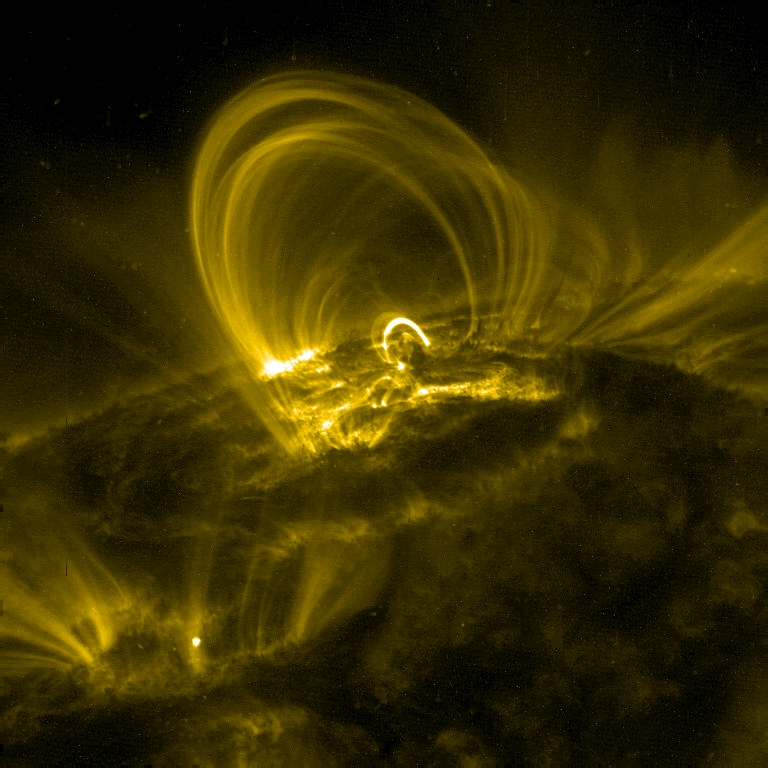
\includegraphics[scale=0.23]{figonea.jpg}
       \caption{ Taken by the {\em Transition Region and Coronal Explorer},
                 (TRACE)---a mission of the Stanford-Lockheed Institute for 
                 Space Research, and part of the NASA small explorer program.
                 \label{fig:figonea}
               }
    \end{subfigure}
%
    \hspace {0.05\textwidth}
%
    \begin{subfigure}[t]{0.45\textwidth}
       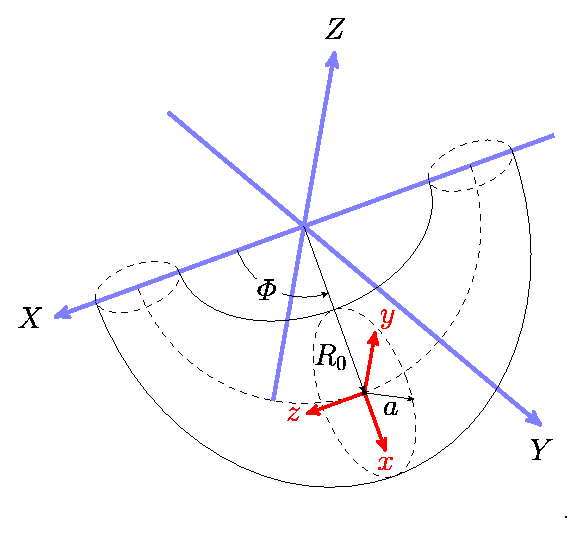
\includegraphics[scale=0.80]{figoneb.eps}
       \caption{Idealized model of a coronal loop.
                \label{fig:figoneb}
               }
    \end{subfigure}
%
    \caption{One application for \coronos: modeling coronal loops.
                \label{fig:figone}}
  \end{figure}
%
% ~~~~~~~~~~~~~~~~~~~~~~~~~~~~~~~~~~~~~~~~~~~~~~~~~~~~~~~~~~~~~~~~~~~~~~~~~~~~ %
%
In the idealized model of a coronal loop shown in figure~\ref{fig:figoneb},
the local Cartesian coordinates $(x,y,z)$ are to be identified with the
dimensionless coordinates appearing in the reduced model examples given below,
and are related to the global cylindrical coordinates $(R,\Phi,Z)$ according
to,
%
\begin{subequations}
	      \begin{align}
		      x   &= (R - R_0)/a \\
		      y   &= Z           \\
		      z   &= -\Phi,
	      \end{align}
\end{subequations}
%
where $R_0$ serves as a characteristic toroidal radius for the loop
center, and $a$ as radius for the loop cross-section.
%
\par
%
To emphasize \coronos\ as a framework for the integration of an entire
class of plasma models, I continue with a rather abstract and unfolding
characterization of what is meant here by the phrase ``Reduced
Plasma Models.''  after which I will provide clarification by citing
a number of examples at least some of which are likely to be familiar
to the reader.
%
In the section following this one, I will revert to the more abstract
description of this class of model in the hope that the reader will
quickly begin to see how the modularization sought in \coronos\ begins
at the level of model specification, and prior to the writing of any lines
of code.
%
In all sections where it is warranted---beginning with this one---a
color-coding standard will be applied so that readers can follow the 
manner in which the representations of the various and distinct features
of these models connect across the analytical and numerical representations
of the models themselves. This approach, though requiring some patience 
on the part of the reader, is intended to help the reader as much as 
possible in grasping the philosophy behind \coronos' design, and to aid in
understanding how the task of expanding \coronos\ to include the 
implementation of additional reduced models is localized and minimized
in the code.
%
\par
%
Let $\pmodel^{(z)}_\epsilon(F_i, G_i; N_f)$ represent a particular reduced
plasma model consisting of $N_f$ model equations which are nonlinear and
coupled, and where the $F_i$ refer to the $N_f$ principle dependent fields
variables to be solved for when integrating the model. Further let the $G_i$
refer to $N_f$ auxiliary fields whose definitions are related to the $F_i$ by
way of a Laplacian operator to be further specified below. Let it additionally
be understood that all fields $F_i$ and $G_i$ are scalar fields depending on
the three Cartesian spatial coordinates $(x,y,z)$ and the time $t$. Let it be
further understood that all field quantities, model parameters, and coordinates
in space and time have been scaled to dimensionless units. 
%
\par
%
Finally, let it be understood that, intrinsic to the model $\pmodel$, is a
``preferred direction'' (specifically $z$ in all cases presented here),
for which there exists a zeroth-order vector quantity (actually a magnetic
``guide'' field, $\Bvec_G=B_0\zhat$), and relative to which variations of
higher order are understood to be the order of some power of an associated
``small parameter'' ($\epsilon$). The guide field $\Bvec_G$ can in, principle
vary with $x$, $y$, and even $z$ though in all cases examined here,
it is simply the unit vector $\zhat$. \footnote{we note here that variation
in $z$ though, necessarily allowable for a full implementation of inhomogeneous
reduced models would require enhancements to the specification of the \coronos'
numerical volume which have not yet been implemented}.
%
\par
%
For any such model $\pmodel$, of the kind defined above, the $i$'th equation of
that model---giving the time-evolution of the field $F^{(i)}$---is expressible
according to,
%
% ~~~~~~~~~~~~~~~~~~~~~~~~~~~~~~~~~~~~~~~~~~~~~~~~~~~~~~~~~~~~~~~~~~~~~~~~~~~~ %
\begin{equation}
  F^{(i)}_t = { \color{red!65!black} B^{(i)}}
            + { \color{blue!65!black} D^{(i)}_z}
            + { \color{green!65!black}G^{(i)}}
            + { \color{orange} L^{(i)}_\perp},
            \label{eq:redmodabs}
\end{equation}
%
where,
%
\begin{subequations}
  \begin{align}
%
   F^{(i)}_t      &=\pardt F^{(i)}                                                                   \\
   B^{(i)}        &=
   \sum_{j \ne k}\epsilon_{ijk}\biggl\{   b^{(F_j,F_k)}_{i,j,k}\left[F^{(j)},F^{(k)}\right] \nonumber \\
                  &\hspace{2cm}       +  b^{(F_j,G_k)}_{i,j,k}\left[F^{(j)},G^{(k)}\right]
                                      +  b^{(G_j,G_k)}_{i,j,k}\left[G^{(j)},G^{(k)}\right]
                                \biggr\}                                                              \\
   D_z^{(i)}      &=\sum_{j} \left\{f_{ij}(z)\pardz F^{(j)} + g_{ij}(z)\pardz G^{(j)}\right\}        \\
   L^{(i)}_\perp  &= c_{F^{(i)}}\delperp^2F^{(i)}.
%
  \end{align}
\end{subequations}
%\begin{list}{\Box}{
%  \setlength{\labelwidth}{5.0 cm}
%  \setlength{\leftmargin}{5.08cm}
%                  }
%%
%   \item[$F^{(i)}_t=\pardt F^{(i)}$\hfill]
%        {is the partial time derivative of the field $F^{(i)}$}
%%
%\item[{\color{red!65!black}$B^{(i)} =
%  \sum_{j \ne k}\epsilon_{ijk}\left\{   b_{F_i,j,k}\left[F^{(j)},F^{(k)}\right]
%                                      + b_{G_i,j,k}\left[G^{(j)},F^{(k)}\right]
%                             \right\}$
%      }
%     \hfill]
%     {is a sum of terms involving Poisson brackets and which together
%      completely specify the nonlinear coupling among fields for the
%      $i$'th equation.
%     }
%
%  \item[{\color{blue!65!black}$D_z^{(i)}$}=\sum{\hfill]{terms involving partial spatial 
%        derivatives in $z$.}
%
%  \item[{\color{green!65!black}$G^{(i)}$}\hfill]{auxiliary term(s) present for some 
%        models}
%
%  \item[{\color{orange}$L^{(i)}_\perp$}\hfill]{dissipative term of the form 
%        $c_{F^{(i)}}\delperp^2F^{(i)}$, where $c_{F^{(i)}}$ is a constant.}
%
%\end{list}
%
% ~~~~~~~~~~~~~~~~~~~~~~~~~~~~~~~~~~~~~~~~~~~~~~~~~~~~~~~~~~~~~~~~~~~~~~~~~~~~ %
%
As a starting example, we consider homogeneous reduced magnetohydrodynamics
(RMHD) \citep{KadomtsevPogutse74, Strauss76, Strauss77}. Developed originally
for the study of fusion plasmas, RMHD is a reduction of incompressible,
resistive magnetohydrodynamics that assumes constant plasma density $n$
and a strong, constant, zero-order guide field of strength $B_0$ (which we
take to lie along $\zhat$). The dynamics of interest occur at first-order
with respect to the guide field, and are restricted to fluctuations
of the magnetic and velocity fields perpendicular to the guide field.
The dynamics thus occur on an \Alfven time scale
$\talfven\sim L/\magvalfven$ where $L$ is some characteristic length scale
for the system and $\magvalfven$ is the \Alfven speed.
%
\par
%
Choosing dimensionless units and the normalization $B_0=\magvalfven=1$, 
we may write the model equations for RMHD according to,
%
\begin{subequations}
\begin{align}
  \pardt\Omega &={\color{red!65!black}-[\phi,\Omega]} + {\color{red!65!black}[A,J]} 
                                                      + {\color{blue!65!black}\pardz J}   
                                                                                        + {\color{orange}\nu \delperp^2\Omega},\label{eq:rmhdvort}  \\
  \pardt A     &={\color{red!65!black}-[\phi,A]}      
                                                      + {\color{blue!65!black}\pardz\phi} 
                                                                                        + {\color{orange}\eta\delperp^2 A}     \label{eq:rmhdflux}.
\end{align}
\end{subequations}
%
The primary field variables in this pair of equations are the $z$-component
of the vorticity $\Omega$, and the poloidal magnetic flux $A$ (to be referred
to more simply in what follows as the ``flux function.'') These variables
are related to the fluctuations in the velocity field $\vvec$ and
the magnetic field $\Bvec$ according to,
%
\begin{subequations}
\begin{align}
  \Bvec        &= \delperp A      \cross \zhat + B_0\zhat \label{eq:rmhdbfroma}      \\
  \Vvec        &= \delperp \Omega \cross \zhat            \label{eq:rmhdvfromomega}.
\end{align}
\end{subequations}
%
In all of equations (\ref{eq:rmhdvort})$-$(\ref{eq:rmhdvfromomega}), the operator
$\delperp$ for some field $F$ is defined according to,
%
\begin{subequations}
\begin{equation}
  \delperp F=\xhat\pardx F + \yhat\pardy F \label{eq:defdelperp}.
\end{equation}
\end{subequations}
%
Auxiliary fields consisting of a ``Stream function'' $\phi$, and
the parallel component of current density $J$ (to be referred to 
henceforth simply as the ``current density''), are then related 
via this operator to $\Omega$ and $A$ respectively according to,
\footnote{In this document we use the sign conventions in 
\citet{Longcope93}. In many other references, the convention
chosen is such that the minus signs appearing here in
equations~(\ref{eq:omegafromphi}) and (\ref{eq:jfroma})
are absent.}
%
\begin{subequations}
\begin{align}
  \Omega &=-\delperp^2\phi  \label{eq:omegafromphi} \\
  J      &=-\delperp^2 A,     \label{eq:jfroma}
\end{align}
\end{subequations}
%
where, for some field $F$, 
%
\begin{subequations}
\begin{equation}
  \delperp^2 F=\delperpdot\delperp F=\parddx F + \parddy F. \label{eq:defdelperpsqd}
\end{equation}
\end{subequations}
%
This ``perpendicular Laplacian operator'' is seen to appear in the
the dissipative terms of equations~(\ref{eq:rmhdvort}) and
(\ref{eq:rmhdflux})  where we also identify the dimensionless
resistivity $\eta$, and dimensionless viscosity $\nu$.
%
Two other types of terms also appear in these equations. We see linear
terms involving partial derivatives in $z$ of the auxiliary fields
$J$ and $\phi$, and we see nonlinear terms expressed as perpendicular
Poisson brackets which we define here for any pair $(f,g)$ of
fields according to,
%
\begin{equation}
  [f,g] = -\zhat \cdot \left(\delperp f\cross\delperp g\right) = \pardy f\pardx g - \pardx f \pardy g.
  \label{eq:pbdef}
\end{equation}
%
Comparing equations~(\ref{eq:rmhdvort}) and (\ref{eq:rmhdflux}) to equation~(\ref{eq:redmodabs}),
            \label{eq:redmodabs}
we identify that for RMHD:
%
\begin{subequations}
\begin{align}
  F^{(0)} &= \Omega  \label{eq:rmhdfzero}                                                              \\
  F^{(1)} &=  A,     \label{eq:rmhdfone}
\end{align}
\end{subequations}
%
\begin{subequations}
\begin{align}
  {\color{red!65!black}B^{(0)}} &= {\color{red!65!black}-[\phi,\Omega]} + {\color{red!65!black}[A,J]} \label{eq:rmhdbzero} \\
  {\color{red!65!black}B^{(1)}} &= {\color{red!65!black}-[\phi,A]},                                    \label{eq:rmhdbone}
\end{align}
\end{subequations}
%                                   
\begin{subequations}
\begin{align}
  {\color{blue!65!black}D^{(0)}} &= {\color{blue!65!black}\pardz J}                                   \label{eq:rmhddzero} \\
  {\color{blue!65!black}D^{(1)}} &= {\color{blue!65!black}\pardz\phi},                                \label{eq:rmhddone}
\end{align}
\end{subequations}
%
\begin{subequations}
\begin{align}
  {\color{orange}L^{(0)}_\perp} &={\color{orange}\nu \delperp^2\Omega} \label{eq:rmhdlzero} \\
  {\color{orange}L^{(1)}_\perp} &={\color{orange}\eta\delperp^2 A},    \label{eq:rmhdlone}
\end{align}
\end{subequations}
%
and,
%
\begin{subequations}
\begin{align}
  {\color{orange}C_{F^{(0)}}} &={\color{orange}\nu }  \label{eq:rmhdczero} \\
  {\color{orange}C_{F^{(1)}}} &={\color{orange}\eta}, \label{eq:rmhdcone}
\end{align}
\end{subequations}
%
while the ``auxiliary terms'' {\color{green!65!black}$G^{(i)}$} are
absent.
%
\par
%
The RMHD model has been extended to account for plasma media with
inhomogeneities in plasma density $n=n(z)$ and zero-order magnetic 
field ($B_0= B_0{z}$), along the guide-field direction 
\citep{HeinemannOlbert80, Vellietal89}.
Typically, this inhomogeneous RMHD (\irmhd) model is expressed in
terms of the \elsasser\ fields $\zvec^\pm$, 
(see for example \citet{PerezChandran2013}). However, because \coronos\
descends from an implementation of RMHD in terms of the fields
$\phi$, $\Omega$, $A$, and $J$, we present the model here in terms
of these.\footnote{This is ultimately because \coronos\ currently 
implements \irmhd in terms of these fields, but the design of \coronos\ allows 
in principle for alternatives, including an \elsasser\ form if desired.}
In terms of these fields then, and using the same definitions
and conventions already adopted above for RMHD, we may write the \irmhd
model according to,
%
\begin{subequations}
%
  \begin{align}
    \pardt\Omega &=
    - {\color{red!65!black}[\phi,\Omega]} + {\color{red!65!black}[A,J]}
    - {\color{blue!65!black}\left[U\pardz\Omega - \magvalfven\pardz J\right]} \nonumber \\ 
    & \qquad\qquad\qquad\qquad\qquad + {\color{green!65!black}\left[\kpm U\Omega - \kpp\magvalfven J\right]} 
    + {\color{orange}\zeta\delperp^2\Omega}
    \label{eq:ihomega}  \\
%
    \pardt A     &=
    - {\color{red!65!black}[\phi,A]}
    - {\color{blue!65!black}\left[U\pardz A  - \magvalfven\pardz\phi\right]}
    + {\color{green!65!black}\left[\kmm U A  - \kmp\magvalfven\phi\right]}
    + {\color{orange}\zeta\delperp^2A}.
    \label{eq:iha}
  \end{align}
\end{subequations}
%
In addition to the quantities already defined for RMHD, some new quantities
appear in these equations. These are the mean flow velocity along $z$ $U=U(z)$,
and a $z$-dependent \Alfven\ speed given in our dimensionless units by,
%
\begin{equation}
  \magvalfven(z)=B_0(z)^2n(z)^{-1/2}.
\end{equation}
%
The quantities $B_0$, $n$, and $\magvalfven$ are related to one
another by way of a steady-state condition given by, \citep{Whang80}
%
\begin{equation}
  \frac{d}{dz}\left(\frac{n(z)U(z)}{B_0(z)}\right) = 0 \label{eq:consflux},
\end{equation}
%
and the four quantities $\kppm$, $\kmpm$ are linear combinations of 
the inverse length scales associated with $n(z)$, $\magvalfven(z)$, and
$B_0(z)$ as follows:
%
\begin{subequations}
\begin{align}
  \kppm &=\frac{1}{2H_B} + \frac{1}{2H_A} \pm \frac{1}{4H_n} \label{eq:kppmdef} \\
  \kmpm &=\frac{1}{2H_B} - \frac{1}{2H_A} \pm \frac{1}{4H_n} \label{eq:kmpmdef},
\end{align}
\end{subequations}
%
where,
%
\begin{subequations}
\begin{align}
  H_n^{-1} &= \left|\frac{1}{n}\frac{\partial n}{\partial z}\right|                     \label{eq:defhr} \\
  H_B^{-1} &= \left|\frac{1}{B_0}\frac{\partial B_0}{\partial z}\right|                 \label{eq:defhb} \\
  H_A^{-1} &= \left|\frac{1}{\magvalfven}\frac{\partial\magvalfven}{\partial z}\right|. \label{eq:defha}
\end{align}
\end{subequations}
%
Finally, the single diffusivity $\zeta$ in this model appears in both
equations, so that in the limits $U\rightarrow 0$, $\magvalfven\rightarrow 1$,
and $\kppm,\kmpm\rightarrow 0$, equations~(\ref{eq:ihomega}) and
(\ref{eq:iha}) reduce to equations~(\ref{eq:rmhdvort}) and (\ref{eq:rmhdflux})
but with $\nu=\eta=\zeta$.
%
\par
%
Specification of $n(z)$, $B_0(z)$, and $\magvalfven(z)$ is non-trivial
and depends on the problem to be studied. We leave the matter to another
section and instead focus on mathematical features of the 
model.\footnote{Variation in $z$ of $B_0$ is particularly problematic as
it requires addressing the issue of magnetic flux conservation along $z$.
At present, the current implementation of \irmhd is limited to cases where
$n$ and $\magvalfven$ may both vary in $z$, but $B_0$ remains constant.}
Referring again to equation~(\ref{eq:redmodabs}) and comparing with
equations~(\ref{eq:ihomega}) and (\ref{eq:iha}) we identify the 
following for \irmhd:
%
\begin{subequations}
\begin{align}
  F^{(0)} &= \Omega                                                                                   \label{eq:irmhdfzero} \\
  F^{(1)} &=  A,                                                                                      \label{eq:irmhdfone}
\end{align}
\end{subequations}
%
\begin{subequations}
\begin{align}
  {\color{red!65!black}B^{(0)}} &= {\color{red!65!black}-[\phi,\Omega]} + {\color{red!65!black}[A,J]} \label{eq:irmhdbzero}  \\
  {\color{red!65!black}B^{(1)}} &= {\color{red!65!black}-[\phi,A]},                                   \label{eq:irmhdbone}
\end{align}
\end{subequations}
%                                   
\begin{subequations}
\begin{align}
  {\color{blue!65!black}D^{(0)}} &= {\color{blue!65!black} -[U\pardz\Omega - \magvalfven\pardz J]}    \label{eq:irmhddzero}   \\
  {\color{blue!65!black}D^{(1)}} &= {\color{blue!65!black} -[U\pardz A     - \magvalfven\pardz\phi]}, \label{eq:irmhddone}
\end{align}
\end{subequations}
%                                   
\begin{subequations}
\begin{align}
  {\color{green!65!black}G^{(0)}} &= {\color{green!65!black} - [\kpm U\Omega - \kpp\magvalfven    J]}    \label{eq:irmhdgzero} \\
  {\color{green!65!black}G^{(1)}} &= {\color{green!65!black} - [\kmm U A     - \kmp\magvalfven \phi]},   \label{eq:irmhdgone}
\end{align}
\end{subequations}
%
\begin{subequations}
\begin{align}
  {\color{orange}L^{(0)}_\perp} &={\color{orange}\zeta\delperp^2\Omega} \label{eq:irmhdlzero} \\
  {\color{orange}L^{(1)}_\perp} &={\color{orange}\zeta\delperp^2 A},    \label{eq:irmhdlone}
\end{align}
\end{subequations}
%
and,
%
\begin{subequations}
\begin{align}
  {\color{orange}C_{F^{(0)}}} &={\color{orange}\zeta}  \label{eq:rmhdczero} \\
  {\color{orange}C_{F^{(1)}}} &={\color{orange}\zeta}, \label{eq:rmhdcone}.
\end{align}
\end{subequations}
%
\par
%
As a third example, and to illustrate that \coronos\ anticipates reduced models
with a larger number of fields, we write the equations for the cold-ion limit of
the 3D four-field equations as presented by \citet{Tassietal2010}. The Four-Field
model was developed to generalize the equations of RMHD to include finite Larmor
radius effects, the adiabatic electron limit, and plasma compressibility.
\citep{Hazeltineetal85,Hazeltineetal87}. The 3D model of \citet{Tassietal2010},
as written using the notation and conventions adopted for this document, and with
dissipative terms added, is as follows:
%
\begin{subequations}
\begin{align}
\pardt \Omega &= - {\color{red!65!black}[\phi,\Omega]}    - {\color{red!65!black}[J,A]}
                 + {\color{blue!65!black} \pardz J}
                 + {\color{orange}\nu\delperp^2   \Omega} \label{eq:ffomega}                           \\
\pardt\hfield &= - {\color{red!65!black}[\phi,\hfield]}   - {\color{red!65!black}d_\beta[A,Z]}
                 + {\color{blue!65!black}\pardz\phi}      - {\color{blue!65!black}d_\beta\pardz Z}
                 + {\color{orange}\eta\delperp^2   A}     \label{eq:ffh}                               \\
\pardt Z      &= - {\color{red!65!black}[\phi,Z]}         - {\color{red!65!black}c_\beta[V,A]} + {\color{red!65!black}d_\beta[J,A]}
                 + {\color{blue!65!black}c_\beta\pardz V} - {\color{blue!65!black}d_\beta\pardz J}
                 + {\color{orange}\kappa\delperp^2 Z}     \label{eq:ffz}                               \\
\pardt V      &= - {\color{red!65!black}[\phi,V]}         - {\color{red!65!black}c_\beta[Z,A]}
                 + {\color{blue!65!black}c_\beta\pardz Z}
                 + {\color{orange}\mu\delperp^2    V}.    \label{eq:ffv}
\end{align}
\end{subequations}
%
The fields, $\phi,$, $\Omega$, $A$, and $J$, are all as defined
above, and we have introduced the additional field quantities,
%
\begin{subequations}
  \begin{align}
    \hfield &= A + d_e^2 J               \label{eq:defh} \\
     Z      &= \zhat\cdot \Bvec/c_\beta  \label{eq:defz} \\
     V      &= \zhat\cdot \Vvec,         \label{eq:defv}
  \end{align}
\end{subequations}
%
where $\Vvec$ and $\Bvec$ are the plasma velocity and magnetic
fields respectively, and the shift to an equation for the
quantity $\hfield$ arises from the inclusion of electron inertia
in the model. Some new parameters also appear in
equations~(\ref{eq:defh})-(\ref{eq:defv}) as well as in
equations~(\ref{eq:ffomega})-(\ref{eq:ffv}). $d_e$  and
$d_i$ are the electron and ion inertial lengths
respectfully, and are related to one another according to,
%
\begin{equation}
  d_e=\sqrt{\frac{m_e}{m_i}} d_i.
\end{equation}
%
The quantities $c_\beta$ and $d_\beta$ are defined by,
%
\begin{subequations}
  \begin{align}
    c_\beta &= \sqrt{\beta/(1+\beta)} \label{eq:defcbeta} \\
    d_\beta &= d_i c_\beta,           \label{eq:defdbeta}
  \end{align}
\end{subequations}
%
where $\beta=(5/3)P_0/B_0^2$, is plasma $\beta$ to lowest order.
Finally, in addition to the diffusivities already defined for RMHD
we have a parallel thermal conductivity $\kappa$ and parallel
viscosity $\mu$ in equations~(\ref{eq:ffz}) and (\ref{eq:ffv})
respectively.
%
\par
%
As before, let us now compare the model given by 
equations~(\ref{eq:ffomega})$-$(\ref{eq:ffv}) to 
equation~(\ref{eq:redmodabs}). Now we identify:
%
\begin{subequations}
\begin{align}
  F^{(0)}                        &= \Omega                                                                             \label{eq:ffzero} \\
  F^{(1)}                        &=  \hfield                                                                           \label{eq:ffone}  \\
  F^{(2)}                        &=  Z                                                                                 \label{eq:fftwo}  \\
  F^{(3)}                        &=  V                                                                                 \label{eq:ffthree}
\end{align}
\end{subequations}
%
\begin{subequations}
\begin{align}
  {\color{red!65!black}B^{(0)}}  &= -{\color{red!65!black}[\phi,\Omega]}  
                                    -{\color{red!65!black}[J,A]}                                             \label{eq:ffbzero} \\
  {\color{red!65!black}B^{(1)}}  &= -{\color{red!65!black}[\phi,\hfield]}
                                    -{\color{red!65!black}d_\beta[A,Z]}                                      \label{eq:ffbone}  \\
  {\color{red!65!black}B^{(2)}}  &= -{\color{red!65!black}[\phi,Z]}       
                                    -{\color{red!65!black}c_\beta[V,A]} + {\color{red!65!black}d_\beta[J,A]} \label{eq:ffbtwo}  \\
  {\color{red!65!black}B^{(3)}}  &= -{\color{red!65!black}[\phi,V]}      
                                    -{\color{red!65!black}c_\beta[Z,A]}                                      \label{eq:ffbthree}
\end{align}
\end{subequations}
%                                   
\begin{subequations}
\begin{align}
  {\color{blue!65!black}D^{(0)}} &=  {\color{blue!65!black} \pardz J }       \label{eq:ffdzero}                       \\
  {\color{blue!65!black}D^{(1)}} &=  {\color{blue!65!black}\pardz\phi}      
                                    -{\color{blue!65!black}d_\beta\pardz Z}  \label{eq:ffdone}                        \\
  {\color{blue!65!black}D^{(2)}} &=  {\color{blue!65!black}c_\beta\pardz V} 
                                    -{\color{blue!65!black}d_\beta\pardz J}  \label{eq:ffdtwo}                        \\
  {\color{blue!65!black}D^{(3)}} &=  {\color{blue!65!black}c_\beta\pardz Z}  \label{eq:ffdthree}
\end{align}
\end{subequations}
%                                   
\begin{subequations}
\begin{align}
  {\color{orange}L^{(0)}_\perp} &= {\color{orange}\nu\delperp^2   \Omega}    \label{eq:fflzero}                       \\
  {\color{orange}L^{(1)}_\perp} &= {\color{orange}\eta\delperp^2   A}        \label{eq:fflone}                        \\
  {\color{orange}L^{(2)}_\perp} &= {\color{orange}\kappa\delperp^2 Z}        \label{eq:ffltwo}                        \\
  {\color{orange}L^{(3)}_\perp} &= {\color{orange}\mu\delperp^2    V}.       \label{eq:fflthree} 
\end{align}
\end{subequations}
%
and,
%
\begin{subequations}
\begin{align}
  {\color{orange}C_{F^{(0)}}}     &= {\color{orange}\nu   } \label{eq:ffczero}    \\
  {\color{orange}C_{F^{(1)}}}     &= {\color{orange}\eta  } \label{eq:ffcone}     \\
  {\color{orange}C_{F^{(2)}}}     &= {\color{orange}\kappa} \label{eq:ffctwo}     \\
  {\color{orange}C_{F^{(3)}}}     &= {\color{orange}\mu.  } \label{eq:ffcthree}
\end{align}
\end{subequations}
%
And we note that---as in the case of RMHD---the auxiliary
terms ${\color{green!65!black}G^{(i)}}$ are absent.
%
\par
%
\chapter{Description Numerical Volume and Integration Methodology}
\chapterprecis{Wherein we introduce the reader to the gist of this document}
%
\begin{figure}[ht]
  \centering
  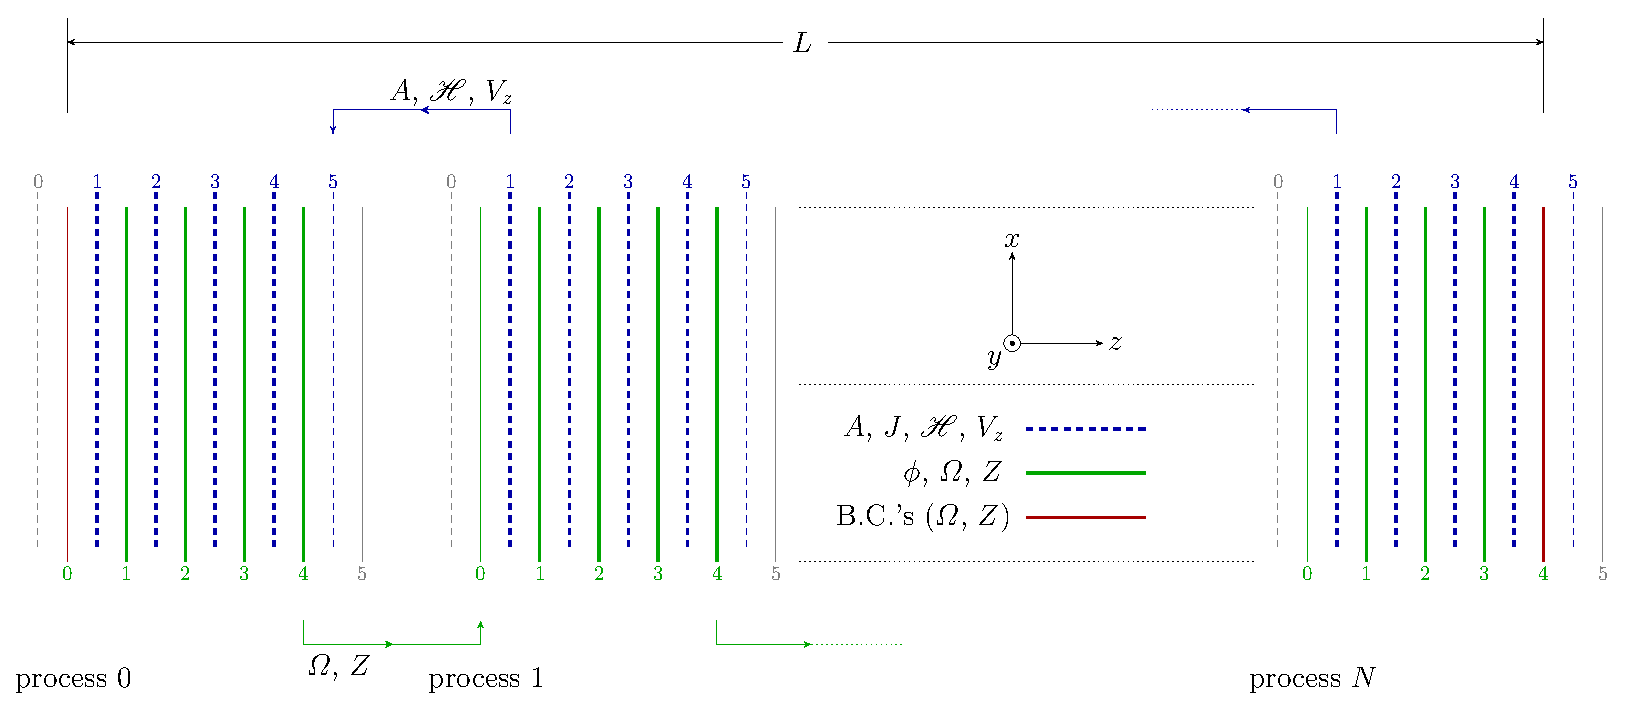
\includegraphics[scale=0.5]{figtwo.eps}
  \caption{Domain decomposition for the case of a domain of length
           $L$ along $z$, transverse side length of $\Lperp=1$, with 
           $N_z=4$ principle layers per process, and $N$ processes.  
           Solid lines indicate layers of ``mesh'' $M_1$ while dashed 
           lines indicate layers of mesh $M_2$ (See text). Currently, 
           boundary conditions are specified on ``ghost'' layer $0$ of 
           process $0$ and principle layer $N_z$ of process $N-1$ for 
           fields defined for $M_1$. Field values on interior boundaries 
           are shared across processes as indicated for finite 
           differencing in $z$. Quantities specified on one grid but 
           needed by the other are averaged across adjacent 
           layers. 
           \label{fig:figtwo}
}
\end{figure}
%
In this section, we discuss the specification of the numerical volume, its
domain decomposition, and the discretization methodology used for all of
the reduced models discussed above.
%
\subsection{Numerical Volume}
\label{sec:thevolume}
%
Figure~\ref{fig:figtwo} illustrates 
how the code divides the numerical volume among $N$ processes, as well as 
how information is organized within each process. The volume is divided into 
a ``stack of stacks.'' In what follows, I refer to a stack associated with
a given process, as a ``process-stack.'' Each process-stack consists of
$N_z$ principle layers, numbered $1$ through $N_z$, as well as two 
additional ``ghost'' layers, numbered $0$, and $N_z+1$, at the ``bottom'' 
and ``top'' ends respectively of each process-stack. The figure
illustrates this for the case $N_z=4$. Note that each process-stack is
actually a pair of interleaved stacks $(M_1,M_2)$, (which I shall
call ``meshes'') with $(\phi,\Omega)$ (and perhaps $Z$) defined on $M_1$,
and $(A, J)$ [ and perhaps $(\hfield, V)$ ] defined on $M_2$.
%
\par
%
Taking the resolution of each layer to  be $ N_x\times N_y$, the
discretization of any of the reduced models discussed above proceeds 
as follows for each process:
%
We define the indices 
%
\begin{subequations}
  \begin{align}
   n_x     &= 1,\ldots,N_x        \\
   n_y     &= 1,\ldots,N_y        \\
   n_z     &= 1,\ldots,N_z,       \\ 
   \ell    &= N_x(n_x - 1) + n_y
\end{align}
\end{subequations}
%
and consider points $(x_\ell,y_\ell)$ located on any one of 
the layers of the process-stack, and with $z$-coordinate
$z_{n_z}$. With these, we define the real-valued column-vector
$\tilde\ufield_n$ to contain our discretized field
values at time-step $n$ in real Cartesian space. For
example, for the field $F^{(i)}$ of some model, we
discretize field values on the layers of a process-stack
according to,
%
\begin{equation}
  F^{(i)}(x,y,z,t) \rightarrow \tilde \ufield^{(i)}_{n,n_z,\ell}
  \equiv F^{(i)}\left(x_\ell,y_\ell, z_{n_z}, t_n\right)
  \label{eq:discretizef}
\end{equation}
%
Note that each such column vector contains $N_R$ elements where,
%
\begin{equation}
  N_R = N_xN_y(N_z+2).
\end{equation}
%
Next, we let the complex-valued column vector $\ufield^{(i)}_n$
contain the Fourier components for each of the $N_z$ layers of 
$\tilde\ufield^{(i)}_{n}$ as determined by discrete, transverse, 
Fast Fourier transform (FFT) which we symbolize as
$\fftperp\{\ldots\}$. Symbolically,
%
\begin{equation}
  \ufield^{(i)}_{n,n_z,\lambda} =
  \ufield^{(i)}_{\lambda}(z_{n_z},t_n) = 
  {\fftperp}_\lambda \left\{\tilde \ufield^{(i)}_{n, n_z} \right\}. \label{eq:fftufieldi}
\end{equation}
%
I.e., at time $t=t_n$, the $\lambda$'th Fourier component for the
values of the field $\tilde\ufield^{(i)}$ in layer $n_z$ is given
by $\ufield^{(i)}_{n,n_z,\lambda}$. The elements of
$\ufield^{(i)}_{n,n_z}$ are specified with the index $\lambda$
rather than $\ell$ because as a practical matter, the number of
elements contained in the column vector $\ufield^{(i)}_n$
defined for a given process-stack is not equal to $N_R$.
This is because $\tilde\ufield^{(i)}_n$ is real-valued, hence
the FFT of each of its layers posesses the symmetry property,
%
\begin{equation}
  \ufield^{(i)}_{n,n_z}\left(k_{x_p}, k_{y_q}\right) = {\ufield^{(i)}_{n,n_z}}^*\left(-k_{x_p},-k_{y_q}\right),
\end{equation}
%
where ``$*$'' indicates complex conjugation, and where
%
\begin{subequations}
  \begin{align}
    k_{x_p} &= \frac{2\pi p}{\Lperp}\qquad -\frac{N_x}{2} < p \le \frac{N_x}{2} \\
    k_{y_q} &= \frac{2\pi q}{\Lperp}\qquad -\frac{N_y}{2} < q \le \frac{N_y}{2}
  \end{align}
\end{subequations}
%
are the discrete $k_x$, and $k_y$ wave-number coordinates
in transverse Fourier space. Because of this symmetry, 
it is standard memory-conserving practice when computing 
discrete real-to-complex FFT's to store only the positive
wave-number portion of the result. For this reason, only
$N_x(N_y/2+1)$ complex elements are needed per layer, so
that $\ufield^{(i)}_n$ contains only $N_C$ elements
where,
%
\begin{equation}
N_C=N_x(N_y/2+1)(N_z+2).
\end{equation}
%
Since, $\ufield^{(i)}_n$, analogously to
$\tilde\ufield^{(i)}_n$, is understood to be a 1-dimensional
column vector containing the discrete Fourier-space components
of the field $F^{(i)}(t_n)$ specified for the $N_z+2$ layers 
of a process-stack, I define the index $\lambda$ over the range,
%
\begin{equation}
1 <\lambda  \le N_x\left(N_y/2+1\right),
\end{equation}
%,
and refer to the coordinates $(k_{x_p},k_{y_q})$ as simply
$(k_{x_\lambda}, k_{y_\lambda})$.\footnote{A technical matter
not taken up here but relevant for implementation, is the
ordering of the elements of $\ufield^{(i)}$ with respect to the
wave-number coordinates $(k_{x_\lambda},k_{y_\lambda})$.
In what follows, whenever point-wise operations are indicated
for elements of column vectors, it should be assumed that this
ordering is accounted for.}
%
Henceforth, except where otherwise noted, all complex-valued
column vectors will be understood to be Fourier-space column
vectors with $N_c$ elements, with Fourier components common to
a layer ordered contiguously. Usually both the index $\lambda$
and the index $n_z$ may be suppressed without loss of clarity.
%
\par
%
\subsection{Model Discretization and Numerical Integration}
\label{sec:themethod}
%
Given the definitions and description provided in
section~\ref{sec:thevolume}, we may now outline the
discretization of any of the reduced models discussed in
section \ref{sec:overview} and the method of integration
used by \coronos\ to evolve them in time.\footnote{We also
remind the reader that the method described here is 
applicable in principle to any set of model equations that
can be expressed in the form given by 
equation~(\ref{eq:redmodabs}).} This method is essentially
that of \citep{Longcope93}, as adapted to the formalism
used here. When illustration is called for, we will use 
\irmhd\ as our model since for this model, every type of
term appearing in equation~(\ref{eq:redmodabs})
is represented.
%
\par
%
We begin by considering the equation for the $i$'th field
of some reduced model as given by,
%
\begin{equation}
  \pardt F^{(i)} = { \color{red!65!black}  B^{(i)}       }
                 + { \color{blue!65!black} D^{(i)}_z     }
                 + { \color{green!65!black}G^{(i)}       }
                 + { \color{orange}        L^{(i)}_\perp }.
\end{equation}
%
We wish to adopt the spatial discretization of $F^{(i)}$ given by
equation (\ref{eq:discretizef}), as well as equivalent spatial
discretizations of all the quantities on the right-hand-side,
and apply a discrete transverse FFT over each layer of the result.
%
\par
%
Before proceeding however, it is well to point out that, in general,
equations of a model that evolve fields defined on $M_1$, require
information about fields defined on $M_2$ and vice versa. This
means that averaging must sometimes be done to obtain suitable
values for these fields on the mesh corresponding to the quantity
being evolved on that mesh. In what follows, we will indicate this
with an overbar. However it's important to realize that averaging
on $M_1$ proceeds differently from averaging on $M_2$. So to be
clear let $Q_1$ be a quantity defined on $M_1$, and let $Q_2$ be
a quantity defined on $M_2$. Then the meanings of $\bar Q_1$
and $\bar Q_2$ are as follows:
%
\begin{align}
  \bar Q_{1,i} &= \frac{Q_{1,i  } + Q_{1,i-1}}{2}\qquad \mathrm{On\ } M_2 \\
  \bar Q_{2,i} &= \frac{Q_{1,i+1} + Q_{1,i  }}{2}\qquad \mathrm{On\ } M_1.
\end{align}
%
This subtlety must be considered again when discussing finite
differences along $z$. For now though, let us proceed with the
FFT.
%
\par
%
We note that, in analogy to the continuous Fourier transform,
the FFT has the property that for each layer $n_z$ of some field
column vector $\tilde Q_n$,
%
\begin{subequations}
\begin{align}
  \fftperp\left\{\pardx \tilde Q_{n,n_z}\right\} &= -i\mathbb{K}_{x} \odot Q_{n,n_z} \label{eq:fftpardx} \\
  \fftperp\left\{\pardy \tilde Q_{n,n_z}\right\} &= -i\mathbb{K}_{y} \odot Q_{n,n_z} \label{eq:fftpardy}.
\end{align}
\end{subequations}
%
In these expressions we have defined the column vectors
$\mathbb{K}_x$ and $\mathbb{K}_y$ to contain the $N_x(N_y/2+1)$
Fourier wave-number coordinates $k_{x_\lambda}$ and $k_{y_\lambda}$
respectively, ordered appropriately according to storage conventions
for the elements of $Q_{n,n_z}$. The operator $\odot$ is
adopted to represent point-wise multiplication of the elements
of these column vectors with the elements of $Q_{n,n_z}$, i.e.
%
\begin{subequations}
\begin{align}
  \left[\mathbb{K}_{x} \odot Q_{n,n_z}\right]_\lambda &= \mathbb{K}_{x,\lambda} Q_{n,n_z,\lambda} \\
  \left[\mathbb{K}_{y} \odot Q_{n,n_z}\right]_\lambda &= \mathbb{K}_{y,\lambda} Q_{n,n_z,\lambda},
\end{align}
\end{subequations}
%
where there is no summation over the index $\lambda$ implied. We note that
equations~(\ref{eq:fftpardx})~and~(\ref{eq:fftpardy}) imply that,
%
\begin{equation}
  \fftperp\left\{\delperp^2 \tilde Q_{n, n_z,\lambda}\right\} = -k^2_\lambda Q_{n,n_z,\lambda},
  \label{eq:fftdelperp}
\end{equation}
%
where,
\begin{equation}
  k^2_\lambda = k_{x_\lambda}^2 + k_{y_\lambda}^2.
\end{equation}
%
\par
%
If we were to now also adopt a first-order explicit finite difference
scheme in time with time-step $\delta t$, we may write the result
of the procedure above as,
%
\begin{equation}
  \ufield_{n+1}^{(i, ex)} = \ufield^{(i)}_n
                         + \delta t
                         \left[
                         {\color{red!65!black}                    \bfield^{(i)}_n}
                         + {\color{blue!65!black}                 \dfield^{(i)}_n}
                         + {\color{green!65!black}                \gfield^{(i)}_n}
                         - {\color{orange}         C_F^{(i)} k^2} \ufield^{(i)}_n
                         \right].
  \label{eq:exstep}
\end{equation}
%
Strictly speaking, we have written this expression only for the
$(n_z, \lambda)$'th element of $\ufield_{n+1}^{(i,ex)}$, however
we may suppress these indices without loss of clarity in what 
follows. Later, we will write final expressions for the method
in the more formal notation described above.
The quantities 
{\color{red!65!black}$\bfield^{(i)}_{n}$},
{\color{blue!65!black}$\dfield^{(i)}_n$}, 
and 
{\color{green!65!black}$\gfield^{(i)}_n$} 
are the Fourier-space equivalents of
{\color{red!65!black}$B^{(i)}$},
{\color{blue!65!black}$D_z^{(i)}$}, and 
{\color{green!65!black}$G^{(i)}$} 
respectively at $t=t_n$, while the term 
{\color{orange}$L^{(i)}_\perp$} has 
been handled using the result in equation~(\ref{eq:fftdelperp}).
%
\par
%
As mentioned above, we use the case of \irmhd\ to illustrate
these terms. First, for the Poisson bracket terms we have,
%
\begin{subequations}
\begin{align}
  {\color{red!65!black}\bfield^{(0)}_n} &= -{\color{red!65!black}[\phi,\Omega]_n} - {\color{red!65!black}[\bar J,\bar A]_n} \label{eq:bdefa} \\
  {\color{red!65!black}\bfield^{(1)}_n} &= -{\color{red!65!black}[\bar\phi,A]_n}.                                           \label{eq:bdefb}
\end{align}
\end{subequations}
%
Here, the bracketed quantities are understood to be the
$(n_z,\lambda)$ elements of the Fourier transforms of
the results obtained from an evaluation of the bracket
made using the ``collocation'' method.\footnote{Also,
where overbars are indicated, the averages are calculated
prior to the evaluation of the bracket.} In this method
the required derivatives for the evaluation of the
bracket are obtained in Fourier space making use of the
property given by equations~(\ref{eq:fftpardx}) and
(\ref{eq:fftpardy}). These are then reverse transformed
into real Cartesian space where they are combined as
prescribed by the definition of the Poisson bracket given
in equation~(\ref{eq:pbdef}). The result is then transformed
back to Fourier space.  For example, for the bracket
{\color{red!65!black}$[X,Y]_{n,n_z}$}, (now regarded as
the section of a column vector corresponding to elements
for layer $n_z$), we would evaluate the required real
space derivatives as follows:
%
\begin{subequations}
\begin{align}
  (\pardx \tilde X)_{n,n_z} &= \fftperp^{-1}\left\{ -i\mathbb{K}_{x} \odot X_{n,n_z}\right\} \\
  (\pardy \tilde X)_{n,n_z} &= \fftperp^{-1}\left\{ -i\mathbb{K}_{y} \odot X_{n,n_z}\right\} \\
  (\pardx \tilde Y)_{n,n_z} &= \fftperp^{-1}\left\{ -i\mathbb{K}_{x} \odot Y_{n,n_z}\right\} \\
  (\pardy \tilde Y)_{n,n_z} &= \fftperp^{-1}\left\{ -i\mathbb{K}_{y} \odot Y_{n,n_z}\right\},
\end{align}
\end{subequations}
%
where $\fftperp^{-1}\{\ldots\}$ indicates reverse Fourier
transform. Then,
%
\begin{equation}
  {\color{red!65!black}[X,Y]_{n,n_z}} = {\color{red!65!black}{\fftperp}
   \left\{   
             (\pardy \tilde X)_{n,nz} \odot (\pardx \tilde Y)_{n,n_z}
           - (\pardx \tilde X)_{n,nz} \odot (\pardy \tilde Y)_{n,n_z} 
  \right\}}.
\end{equation}
%
\par
%
The second term inside the brackets of equation~(\ref{eq:exstep})
represents all terms containing partial derivatives in $z$. For the
case of \irmhd, we would write,
%
\begin{subequations}
\begin{align}
%
  {\color{blue!65!black}\dfield^{(0)}_{n,n_z}} &= 
%
  {\color{blue!65!black}
     \magvalfven(z_{n_z})\left(\frac{\Delta  J}{\Delta z}\right)_{n,n_z} 
    - U(z_{n_z})\left(\frac{\Delta \Omega}{\Delta z}\right)_{n,n_z}
  } \label{eq:ddefa} \\
%
  {\color{blue!65!black}\dfield^{(1)}_{n,n_z}} &= 
%
  {\color{blue!65!black}
    \magvalfven(z_{n_z})\left(\frac{\Delta \phi}{\Delta z}\right)_{n,n_z}
   - U(z_{n_z})\left(\frac{\Delta A}{\Delta z}\right)_{n,n_z}
  },\label{eq:ddefb}
%
\end{align}
\end{subequations}
%
Where we have made the index $n_z$ explicit in equations~(\ref{eq:ddefa})
and (\ref{eq:ddefb}) because of the $z$-dependence of the quantities
$\magvalfven$ and $U$.
%
\par
%
We've previously pointed out that choosing some fields to be defined on
$M_1$ and others to be defined on $M_2$ requires averaging when information
on one of the meshes is needed on the other. This subtletly arises again
when choosing our discretization for the finite difference. We may infer
from figure~\ref{fig:figtwo} how second-order spatial finite differencing
in $z$ is accomplished. When, at some time-step $n$, a grid-layer located
at, say $z_{n_z}$, requires the evaluation of a finite difference of some
field quantity $X_n$, the finite difference is carried out according to
one of the following,
%
\begin{subequations}
\begin{eqnarray}
  \left(\frac{\Delta X_2}{\Delta z}\right)_n &= \left(\frac{X_{1,n,n_z+1} - X_{1,n,n_z  }}{z_{1,n_z+1}-z_{1,n_z  }}\right) 
  \label{eq:fda} \\
  \left(\frac{\Delta X_1}{\Delta z}\right)_n &= \left(\frac{X_{2,n,n_z}   - X_{2,n,n_z-1}}{z_{2,n_z}  -z_{2,n_z-1}}\right)
  \label{eq:fdb}
\end{eqnarray}
\end{subequations}
%
Note that indices are provided for both $X$ and $z$ to indicate both
the layer on a mesh (i.e., $n_z$) as well as the particular mesh upon
which information about the quantity the quantity is needed. We can
simplify this somewhat by noting that although the layers of $M_1$
are always {\em logically} staggered with respect to those of $M_2$,
\textit{ they are not necessarily spatially staggered}. If the layers
are distributed uniformly in $z$, it follows that,
%
\begin{equation}
  \Delta z = (z_{n_z+1}-z_{n_z}) = (z_{n_z} - z_{n_z-1}),
\end{equation}
%
so that the denominators above may henceforth be written simply
as $\Delta z$. 
%
\par
%
From the point of view of second-order accuracy however, the
distinction between grids is still important.  When finite
differences involving \textit{$X$ defined on $M_2$} are
needed \textit{on layer $n_z$ of $M_1$} they are evaluated
using~equation~(\ref{eq:fda}), and when finite differences
\textit{involving $X$ defined on $M_1$} are needed
\textit{on layer $n_z$ of $M_2$} they are evaluated using
equation~(\ref{eq:fdb}). These are straightforward when
the finite difference in question involves a field $X$
which is defined on the ``complementary'' grid as just
described. For example, the finite difference in $J$
needed for the update, $\ufield^{(0)}_{n+1}$, is readily
evaluated since $\ufield^{(0)}_{n+1}$ is defined on $M_1$
while $J_{n,n_z+1}$ and $J_{n,n_z}$ are both defined
on $M_2$.
%
\par 
%
For \hrmhd, (and for \irmhd\ in the absence of a mean flow)
this is the only finite difference required for the vorticity
equation. However, when there is a mean flow, the vorticity
equation also requires the evaluation of a finite difference
in $\Omega$ which is not defined on layers $n_z$ and $n_z+1$
of $M_2$. To get around this problem, we calculate the average
of $\Omega$ across the pair of layers $(n_z-1,n_z)$ on
grid $M_1$ to obtain suitable value of $\Omega_{n,n_z}$ on
$M_2$ and across the pair of layers $(n_z,n_z+1)$ on $M_1$
to obtain a suitable value for $\Omega_{n,n_z+1}$ on $M_2$.
Then we can calculate the finite difference as above. A similar
averaging must be done for the finite difference in $A$
needed for the $\ufield_{i=1,n+1}$ update when there is a
mean flow. The averaging is across the same set of layer-pairs
$(n_z-1,n_z)$ and $(n_z,n_z+1)$, but these now result in
$G_1$-defined values for $A_{n,n_z-1}$ and $A_{n,n_z}$
respectively. Whether on $G_1$ or $G_2$ these averagings
lead to a finite difference of the form,
%
\begin{equation}
  \left(\frac{\Delta \bar X}{\Delta z}\right)_n = \left(\frac{X_{n_z + 1} - X_{n_z-1}}{2\Delta z}\right).
  \label{eq:fdave}
\end{equation}
%
I.e. where an overbar appears above a field quantity in a finite
difference, the finite difference must be evaluated using
equation~(\ref{eq:fdave}), and when the overbar is absent then
we must use one of equations~(\ref{eq:fda})~or~(\ref{eq:fdb}),
with the choice depending on upon which mesh the field quantity
being differenced is defined.
%
\par
%
With this understood, it is best to now rewrite
equations~(\ref{eq:ddefa})~and~(\ref{eq:ddefb}) as,
%
\begin{subequations}
\begin{align}
%
  {\color{blue!65!black}\dfield^{(0)}_{n,n_z}} &= 
%
  {\color{blue!65!black}
     \magvalfven(z_{n_z})\left(\frac{\Delta  J}{\Delta z}\right)_{n,n_z} 
    - U(z_{n_z})\left(\frac{\Delta \bar\Omega}{\Delta z}\right)_{n,n_z}
  } \label{eq:ddefa} \\
%
  {\color{blue!65!black}\dfield^{(1)}_{n,n_z}} &= 
%
  {\color{blue!65!black}
    \magvalfven(z_{n_z})\left(\frac{\Delta \phi}{\Delta z}\right)_{n,n_z}
   - U(z_{n_z})\left(\frac{\Delta \bar A}{\Delta z}\right)_{n,n_z}
  },\label{eq:ddefb}
%
\end{align}
\end{subequations}
%
\par
%
The third term inside the brackets of equation~(\ref{eq:exstep}) collects 
terms with linear dependence on the fields themselves,
%
\begin{subequations}
\begin{align}
%
  { \color{green!65!black}\gfield^{(0)}_{n,n_z}} &= 
%
  {\color{green!65!black}
    U(z_{n_z})\kpm(z_{n_z})\Omega_{n,n_z} - \magvalfven(z_{n_z})\kpp(z_{n_{z}}) J_{n,n_z}   
  } 
  \label{eq:ldefa} \\
%
  {\color{green!65!black}\gfield^{(1)}_{n,n_z}} &= 
%
  {\color{green!65!black}
    U(z_{n_z})\kmm(z_{n_z}) A_{n,n_z}     - \magvalfven(z_{n_z})\kmp(z_{n_z})  \phi_{n,n_z} 
  } 
   \label{eq:ldefb}
%
\end{align}
\end{subequations}
%
Once again, we note that because the quantity-pairs mentioned above are
defined for separate grids, the evaluation of the 
{\color{green!65!black}$\gfield^{(i)}_{n,n_z}$}-terms 
must be considered carefully. We shall discuss this at greater length 
below as well. 
%
\par
%
Finally, the fourth term inside the brackets of equation~(\ref{eq:exstep})
simply represents the Fourier transform of the dissipative terms. We take a
moment to note that in this term as well as in the term outside the brackets
of equation (\ref{eq:exstep}), and in what follows; when one sees
``$\ufield^{(i)}_n$'' without any other superscripts, it refers simply to 
the values of the discretized fields, for all $n_z$ and $\lambda$, at 
time-step $n$ which are presumed known when commencing time-step $n+1$.
%
\par
%
With these same definitions, we can also write the semi-implicit form,
%
\begin{equation}
  \ufield_{n+1}^{(i,im)} = \ufield^{(i)}_n
  + \delta t\left[
                    {\color{red!65!black}  \bfield^{(i)}_n}
                  + {\color{blue!65!black} \dfield^{(i)}_n}
                  + {\color{green!65!black}\gfield^{(i)}_n}
                  - {\color{orange}C^{(i)}_F k^2}
                  \ufield^{(i)}_{n+1}
           \right].
  \label{eq:imstep}
\end{equation}
%
For the time-step in $\delta t$, I now introduce the free,
empirically-chosen, parameters $s_i\in (0,1)$---one for
each component of $\ufield$---and use them to write a new
expression for the $\ufield^{(i)}_{n+1}$ as a hybrid of the
explicit and semi-implicit finite differences given above:
%
\begin{equation}
  \ufield^{(i)}_{n+1} = s_i\ufield^{(i,im)}_{n+1} + (1-s_i)\ufield^{(i,ex)}_{n+1}.
\end{equation}
%
using the expressions given in equations~(\ref{eq:exstep})~
and~(\ref{eq:imstep}) for the $\ufield_i$'s, this becomes,
after some manipulation,
%
\begin{multline}
  \ufield^{(i)}_{n+1} = \biggl\{
%
   \left[
            1 
            - {\color{orange}\left(1-s_i\right)C^{(i)}_F\delta t k^2}
  \right] 
%
  \ufield^{(i)}_n 
  + \\
  \delta t\left[
                  {\color{red!65!black}  \bfield^{(i)}_n}
                + {\color{blue!65!black} \dfield^{(i)}_n}
                + {\color{green!65!black}\gfield^{(i)}_n}
         \right]
                    \biggr\}
   \left[      1
   + {\color{orange}s_iC^{(i)}_F\delta t k^2}
  \right]^{-1}
\end{multline}
%
To ensure second-order accuracy in time, the scheme applies this
differencing twice; once with time step $\delta t = f\Delta t\equiv\Delta t_p$ 
where $f\in (0,1)$, and using evaluations of the quantities 
{\color{red!65!black}$\bfield$},
{\color{blue!65!black}$\dfield$}, 
and 
{\color{green!65!black}$\gfield$} 
based on the field values obtained at the end of time-step $n$; 
and once again for the full time step $\delta t= \Delta t$, 
this time using evaluations of the quantities
{\color{red!65!black}$\bfield$},
{\color{blue!65!black}$\dfield$}, 
and 
{\color{green!65!black}$\gfield$} 
based on field values obtained from the predictor step. 
We distinguish these latter evaluations from the former 
evaluations with a subscripted ``$(p)$'' and write,
%
\begin{subequations}
\begin{align}
  \ufield_{(p),n+1}^{(i)} &= \biggl\{
  \left[ 1 - {\color{orange}\left(1-s_i\right)C^{(i)}_F \Delta t_p k^2}\right] \ufield^{(i)}_n  \nonumber \\
  &\qquad + \Delta t\left[ {\color{red!65!black}\bfield^{(i)}_n} +
  {\color{blue!65!black}\dfield^{(i)}_n}+{\color{green!65!black}\gfield^{(i)}_n}\right]
                    \biggr\}
                    \left[1+{\color{orange}s_iC^{(i)}_F \Delta t_p k^2}\right]^{-1} \\
  \ufield_{(c),n+1}^{(i)} &= \biggl\{
  \left[ 1 - {\color{orange}\left(1-s_i\right)C^{(i)}_F f\Delta t k^2}\right] \ufield^{(i)}_n  \nonumber \\
  &\qquad + \Delta t\left[{\color{red!65!black}\bfield^{(i)}_{(p),n}} +
  {\color{blue!65!black}\dfield^{(i)}_{(p),n}}+{\color{green!65!black}\gfield^{(i)}_{(p),n}}\right]
                    \biggr\}
                    \left[1+{\color{orange}s_iC^{(i)}_F f\Delta t k^2}\right]^{-1}
\end{align}
\end{subequations}
%
These expressions are valid in transverse Fourier space for 
some point $(k_{x_\lambda},k_{y_\lambda})$ on a layer of 
the domain located at $z=z_{n_z}$. To write them in a way
that accounts for all points on a layer, and for all layers, 
let us define vectors,
%
\begin{subequations}
\begin{align}
  { \color{orange} S^{(ex,i)}_{(p)} }  &= {\color{orange}[\mathbb{1} - g^{(ex,i)}_{p} \mathbb{K}^{(2)}]      }  \label{eq:defsexp} \\
  { \color{orange} S^{(im,i)}_{(p)} }  &= {\color{orange}[\mathbb{1} + g^{(im,i)}_{p} \mathbb{K}^{(2)}]^{-1} }  \label{eq:defsimp} \\
  { \color{orange} S^{(ex;(i)}_{(c)} } &= {\color{orange}[\mathbb{1} - g^{(ex,i)}_{c} \mathbb{K}^{(2)}]      }  \label{eq:defsexc} \\
  { \color{orange} S^{(im;(i)}_{(c)} } &= {\color{orange}[\mathbb{1} + g^{(im,i)}_{c} \mathbb{K}^{(2)}]^{-1} }, \label{eq:defsimc}
\end{align}
\end{subequations}
%
with,
%
\begin{subequations}
\begin{align}
  {\color{orange}g^{(ex,i)}_{p}} &= {\color{orange}(1-s_i)C^{(i)}_F \Delta t_p} \label{eq:defgexp} \\
  {\color{orange}g^{(im,i)}_{p}} &= {\color{orange}   s_i C^{(i)}_F \Delta t_p} \label{eq:defgimp} \\
  {\color{orange}g^{(ex,i)}_{c}} &= {\color{orange}(1-s_i)C^{(i)}_F \Delta t  } \label{eq:defexc}  \\
  {\color{orange}g^{(im,i)}_{c}} &= {\color{orange}   s_i C^{(i)}_F \Delta t  },\label{eq:defimc}
\end{align}
\end{subequations}
%
and where,
%
\begin{equation}
  \kcolvec_{(n_z - 1)N_x(N_y/2+1) + \lambda} = k^2_\lambda;\qquad 0\le n_z \le N_z+2.
  \label{eq:defkcol}
\end{equation}
%
That is, $\kcolvec$ is a 1-dimensional column vector with $N_C$
elements, containing $N_z+2$ contiguous ``copies'' of the column
vector containing the quantities $k^2_\lambda$. Also we have defined
$\mathbb{1}$ to be a column vector of the same size as $\kcolvec$
with all elements set to unity. Note that these definitions suffice 
to specify dimensions of the column vectors defined in
equations~(\ref{eq:defsexp})$-$(\ref{eq:defsimc}) as well.
%
\par
%
Now, we may express the entire scheme for all layers of a 
process-stack and for the $(n+1)$'th time-step very compactly
using our notation for point-wise multiplication of column-vectors:
%
\begin{subequations}
\begin{align}
  U^{(i)}_{(p),n+1} &= 
  \biggl\{ 
%
            {\color{orange}S^{(ex,i)}_{(p)} } 
            \odot 
            U^{(i)}_n
%
  + \Delta t_p
    \left[
              { \color{red!65!black}   \bfield^{(i)}_n}
            + { \color{blue!65!black}  \dfield^{(i)}_n}
            + { \color{green!65!black} \gfield^{(i)}_n}
    \right]
 \biggr\} \odot 
%
{\color{orange} S^{(im,i)}_{(p)} }
%
 \label{eq:cipred}  \\
%
  U^{(i)}_{(c),n+1} &= 
   \biggl\{ 
%
 {\color{orange}S^{(ex,i)}_{(c)} }
             \odot 
             U^{(i)}_n
%
  + \Delta t 
    \left[
              {\color{red!65!black}  \bfield^{(i)}_{(p),n} }
            + {\color{blue!65!black} \dfield^{(i)}_{(p),n} }
            + {\color{green!65!black}\gfield^{(i)}_{(p),n} }
    \right]
  \biggr\} \odot 
% %
  {\color{orange}S^{(im,i)}_{(c)} }
  \label{eq:cicorr},
\end{align}
\end{subequations}
%
As indicated by the figure, each of $M_1$, and $M_2$ consists of a total
of $\mathtt{p3}+2$ layers per process.  The ``principle'' layers of
each grid are those with indices ranging from $1$ to $\mathtt{p3}$,
while layers $0$ and $\mathtt{p3}+1$ serve special purposes. These ``ghost''
layers are for the imposition of boundary conditions in the case of
processes with exterior boundaries as well as for communication across
processes when interior boundary layers of one grid require information
from an adjacent layer of the other grid. This communication is as
indicated in the figure. Note that each grid has a single extraneous layer. 
For $G_1$ this layer is at the top of the grid, while for $G_2$ it is at 
the bottom. In the figure they are colored gray to indicate that they
are superfluous.  These layers are present merely to indicate the
manner in which the field-carrying vector $\ufield$ is implemented in
the code. (Currently the code makes no use of this ``wasted'' memory,
though, with some care taken, it could be made to.)
%
\par
%
The relevant ghost layer on $G_1$ for any process occurs at the
bottom. For the process of rank $r_p=0$ this layer is an exterior
boundary and is used for setting boundary conditions. For all other
processes this layer receives its field values from layer $\mathtt{p3}$
of the $G_1$ grid instantiated on the process of rank $r_p-1$ as
indicated in the figure. In contrast, the relevant ghost layer
on $G_2$ occurs at the top. Though in principle it could be used
for setting an upper exterior boundary condition on the $G_2$
grid of process $N-1$, in its current form the code in fact
sets an upper boundary condition on layer $4$ of $G_1$---i.e.
the exterior boundary conditions at both ends are conditions on the 
field $\Omega$ (or equivalently $\phi$). In the figure, the layers
upon which exterior boundary conditions are imposed are colored red.
%
\chapter{Initial Conditions and Boundary Conditions}
\chapterprecis{Wherein we introduce the reader to the gist of this document}
%
\chapter{An Illustration: Modeling Magnetic Reconnection in Homogeneous Reduced MHD}
\chapterprecis{Wherein we introduce the reader to the gist of this document}
%
\chapter{Reduced Model Conservation Laws and Post-Processing Diagnostics}
\chapterprecis{Wherein we introduce the reader to the gist of this document}
%
\chapter{Suggested Protocols for Adapting and Expanding \coronos}
\chapterprecis{Wherein we introduce the reader to the gist of this document}
%
\chapter{Remarks On The Current State of \coronos\ and Essential Tasks Remaining.}
\chapterprecis{Wherein we introduce the reader to the gist of this document}
%
\appendix
\chapter{Appendices}
\chapterprecis{Wherein we introduce the reader to the gist of this document}
\section{A}
\subsection{A i}
\subsection{A ii}
\section{B}
\backmatter
\bibliographystyle{apalike}
\bibliography{turb}{}
%
\end{document}
